\chapter{Numerical Analysis}
The target of Han and Wong was to prove the existence of a solution to the optimisation problem and to prove how roughening the models helps to achieve better outcomes in mean-variance portfolio optimisation problems. We recall the equations we are trying to optimize with \ref{problem_of_portfolio}. 

For that reason, we will focus in this chapter on how to simulate stochastic processes that are markovian (represented by flows), as well as the solution to the optimization problem. Later, we will focus on introducing roughness in the models. That way, we will be able to compare both models' impact upon mean-variance strategies. 

At the end of the chapter, we will know how to generate all the images from the paper \cite{HanWong}. 

\begin{itemize}
\item For graphs 1. (a) and (b) as well as for 2. (a) and (b) please check \ref{SDES},
\item For graph 5. (a) please refer to \ref{processes},
\item For 3. (a), (b); 4. (a), (b), (c) check \ref{rough}.
\end{itemize}


Let's first introduce the different equations we are going to simulate.

\section{Equations considered by Han Wong}

The model we consider is called the Volterra-Heston Model defined by:

\begin{align}
\label{eq:model1}
V_t 
&= V_0 + \kappa \int_0^t  K(t-s)   (  \phi - V_s ) ds + \int_0^t  K(t-s) \sigma \sqrt{V_s} dB_s \\
\label{eq:model2}
d S_t 
&= S_t r_t  dt + S_t \sqrt{V_t} d W_{1,t}, \quad S_0 > 0 \\
\label{eq:model3}
d B_t 
&= \rho d W_{1,t} + \sqrt{1- \rho^2 } d W_{2,t}
\end{align}

where the parameters are described as
\begin{itemize}
\item $V_0 > 0$, starting variance and $S_0 > 0$, starting price,
\item $\kappa > 0$, mean-reversion speed,
\item $\phi >0$, long-term variance,
\item $\sigma > 0$, vol of vol, the volatility of variance of the asset,
\item $r$ risk free interest rates, that we have taken constant throughout that paper. It wouldn't be too difficult to change it to a function, as long as it is deterministic and bounded,
\item $\rho$ constant, correlation between the two Brownian motion $ W_{1,t}$ and $W_{2,t}$,
\item $T$, the maturity.
\end{itemize}

Also, $K$ is a kernel. Classical kernels are given by table \ref{tab:kernels}. We are going to mainly use the power-law one, where for $\alpha = 1$, the model reduces to classical Heston. For $\alpha < 1$, one observes that the model is the Rough Heston model.



\begin{table}
\begin{center}
\begin{tabular}{   m{4.5 cm}  m{4.5 cm}   } 
\hline
 Name  & $K(t)$  \\ 
\hline
Constant & $c$ \\ 
Fractional (Power-law) & $c \frac{t^{\alpha - 1}} {\Gamma(\alpha) }$ \\ 
Exponential & $\alpha e^{-\beta t }$ \\
\hline
\end{tabular}
\caption{Examples of kernels, where $c$ is a constant.}
\label{tab:kernels}
\end{center}
\end{table}


We add to the previous equations a slight modification. We use Girsanov's theorem, in order to change the measure in the following way, where $\theta \neq 0$:


\begin{equation}
\frac{d \mathbb {\widetilde P} } { d \mathbb P} \bigg\rvert_{\mathcal F_t} = \exp \left ( - 2 \theta^2 \int_0^t V_s ds - 2 \theta \int_0^t \sqrt{V_s} d W_{1,s}  \right )
\end{equation}


which then, transforms our equations into their final form:

\begin{align}
V_t &= V_0 + \int_0^t  K(t-s) ( \kappa \phi - \lambda V_s ) ds + \int_0^t  K(t-s) \sigma \sqrt{V_s} d \widetilde{B_s}  \label{eq:original_problem1} \\
d \widetilde{B_s } &:= \rho d [ W_{1,s} + 2 \theta \int_0^s \sqrt{ V_u } du ] + \sqrt{ 1 - \rho^2 } d W_{2,s}  \label{eq:original_problem2} \\
d S_t &= S_t ( r_t + \theta V_t ) dt + S_t \sqrt{V_t} d W_{1,t}, \quad S_0 > 0 \label{eq:original_problem3}
\end{align}

where we also have introduced the new constant $ \lambda = \kappa + 2 \theta \rho \sigma$.

On the other side, we introduce the dynamic of the wealth. It is crucial for our problem as we will try to minimize its volatility while keeping its mean at its highest.
\begin{align}
\label{eq:wealth_process}
d X_t 
&= \left ( r_t X_t + \theta \sqrt{ V_t } u_t \right ) dt + u_t d W_{1,t}, \quad X_0 = x_0 > 0
\end{align}


Finaly, we define an investment strategy, with $\pi_t$ the investment at time $t$ as

\begin{equation}
u_t := \sqrt{V_t} \pi_t 
\end{equation}

and as mentioned in \cite{HanWong}, we restrict the set of strategies to the admissible strategies:

\begin{definition}[admissible strategy]
$u$ is admissible if and only if \\
$\quad$ 1. $u(\cdot)$ is $\mathbb F$-adapted.  \\
$\quad$ 2. $\mathbb E[ (\int_0^T  \sqrt {V_t} u_t dt )^2 ] < \infty$ \\
\quad 3. $\mathbb E[ \int^T_0 u_t^2 dt ] < \infty $ \\
\quad 4. \ref{eq:wealth_process} admits a unique solution in the sense of \cite{ref_hanwong}, chapter $1$ definition $6.15$ with $\mathbb P$-a.s. continuous paths.
\end{definition}

Those restrictions are essential. Hypothesis (1) guaranties that the process is well defined by asking it to be adapted to the natural filtration, hypothesis (2) and (3) guaranty that the computations are bounded\footnote{(3) implies integrability of the portfolio.} and actually those are usual hypothesis applied on strategies. Finally, (4) is imposed for theoritical reasons.

If one denotes by $\mathcal U$ the set of all admissible investment strategies, then the problem of the optimal mean-variance portfolio in continuous time reduces to:


\begin{theoreme}{ Mean-Variance portfolio optimisation problem}
\begin{equation*}
\label{problem_of_portfolio}
\begin{array}{lc}
\Min_{ u \in  \mathcal U }  & J(x_0, u) = \mathbb E [ ( X_T - c )^2 ]          \\
\text{subject to }   & \mathbb E [ X_T ] = c                             \\
                     & (X(\cdot), u(\cdot)) \text{ satisfies (\ref{eq:wealth_process})   }
\end{array}
\end{equation*}
\end{theoreme}

where, in an obvious way the target wealth level $c$, has to be chosen such that:
$$ x_0 e^{ \int_0^T  r_s ds } \leq c $$
otherwise the trivial strategy would give a better solution than the one expected. 

The solution to the previous problem, as proven in \cite{HanWong}, is the following strategy:

\begin{align}
u^* 
&:= A_t 
\sqrt{ V_t} 
\left ( \zeta^* \exp \left ( - \int_t^T r_s ds \right )  - X_t^* \right )  \label{eq:optimal_solution} \\
A_t 
&:= \left ( \theta + \rho \sigma \psi( T-t) \right ) \label{eq:At} \\
\zeta^* 
&:= c - \eta^* = c - \frac{
M_0 x_0 \exp \left ( -  \int_0^T r_s ds \right ) 
- M_0 c \exp \left ( -  \int_0^T 2 r_s ds \right )
}{
2 - M_0 \exp \left ( - \int_0^T 2 r_s ds  \right )
} \\
M_0 &= 2 \exp \left [ \int^T_0 2 r_s ds + \int_0^T \psi(s) ds + V_0 \int^T_0 [ \frac{\sigma^2 ( 1 - 2 \rho^2 ) }{2} \psi^2 ( s) - \lambda \psi (s) - \theta^2 ] ds \right ] \\
\psi(t) &:= \int_0^t K(t-s) \left [ \frac{\sigma^2 ( 1 - 2 \rho^2 ) }{2} \psi^2 ( s) - \lambda \psi (s) - \theta^2 \right ] ds \label{eq:ori_psi}
\end{align}

We didn't write $M_t$, but only $M_0$, since one doesn't need to simulate $M_t$ for getting the optimal strategy.



Finally, under the existence of a solution and regularity condition, the variance of the optimal wealth process is given by (equation (4.32) in \cite{HanWong}): 

\begin{align}
\label{eq:variance_process}
\Var ( X_T^* ) 
&= \frac{ M_0} { 2 - M_0 \exp \left ( - \int_0^T 2 r_s ds  \right ) } ( c \exp \left ( -  \int_0^T r_s ds \right ) - x_0 )^2
\end{align}


We are now going to simulate all those required quantities and processes. We start by solving the Riccati-Volterra equation (\ref{eq:ori_psi}) numerically.

\begin{remarque}
Hereinafter, we shall use the power law kernel as our standard. Recall that it is defined as:
$$ K_{\alpha}(t) = \frac{t^{\alpha - 1 }  }{ \Gamma( \alpha ) }$$

When the result can be generalized for a different kernel, we will write it as a nota bene.
\end{remarque}

\begin{remarque}
Eq. (\ref{eq:ori_psi}) leads the trivial solution (null everywhere) when $\theta$ is taken as zero. If one desire to set $\theta$ as zero, then under the normal Heston ($\alpha = 1$), the equation reduces to a differential equation classified as a "Bernouilli" equation. In the non-trivial kernel case, it is more complicated. Those equations allow a closed form solution, which is non-trivial for a non-zero initial condition. The solution to the equation, which can be written in flow form by the fact that under the last assumptions it became markovian, is then given by the following theorem:
\end{remarque}

\begin{theoreme}{Bernouilli Diff. Eq.'s solution }
The equation : 
$$\psi ' = \frac{(1 - 2 \rho ^2) \sigma ^2}{2}  \psi ^2 - \lambda \psi $$
with boundary condition $\psi(0) = \psi_0 $  has the following solution :

$$ \psi^* (t) = \psi_0 \frac { e^{ - \lambda t } } 
{  1 - \frac {\psi_0}{\lambda}   \left ( \frac{(1 - 2 \rho ^2) \sigma ^2}{2} ( 1 - e^{- \lambda t } ) \right )
}  $$
\end{theoreme}



\section{Simulating SDEs }

\subsection{Fractional Integral}
Under the power-law kernel, one can identify the integrals in the previously stated equations to be fractional integrals. For that reason, methods from fractional integration can be used to compute explicitly the integrals: e.g. in \cite{HanWong}, the authors recommend the use of differeint: "$\text{Available at https://github.com/differint/differint}$". 

Known as Cauchy formula for repeated integration, the formula allows to extend integration to non-integer numbers (even complex numbers).

\begin{theoreme}{Cauchy formula for repeated integration}
$f$, a continuous function over $\mathbb R$, $\alpha \in \mathbb C$, then:
$$
f^{( - \alpha )} (x) = \frac 1 {\Gamma (\alpha)} \int_0^x (x-t)^{\alpha - 1} f(t) dt 
$$

where by $f^{( - \alpha )} $ I mean the $\alpha$-th order integral of $f$, by extension of the notation of $f^{ \alpha}$, the $\alpha$-th order derivative.
\end{theoreme}

I found that using numerical integration method (cf. section \ref{integration}) works as precisely, even though slower.










\subsection{Fractional Adams method}

The fractional Adams method allows to solve numerically equations of the form of the Volterra equation:

$$ h(a,t) = \frac 1 { \Gamma(\alpha)} \int_0^t (t-s)^{\alpha - 1} F ( a, h(a,s) ) ds $$

which equation corresponds to our problem as long as the kernel is chosen as a power-law kernel. Also $a$ is either a parameter, or a set of parameters.

Good information about the scheme can be found in \cite{Euch} section 5.1, \cite{Diethelm1}, \cite{Diethelm2}. Convergence is proven in \cite{convergence_psi}.

The idea goes as follows. 

We introduce a regular discrete time-grid $(t_j)$ with mesh $\delta$ ( i.e. $t_j = j \Delta$). 

Recursively, over the time-grid, we want to compute:

$$ h(a,t_{k+1} ) = \frac 1 { \Gamma(\alpha)} \int_0^{t_{k+1}} (t_{k+1}-s)^{\alpha - 1} F ( a, h(a,s) ) ds $$ 

Firstly, we approximate the integrand by:

$$ h(a, t) = \frac 1 { \Gamma(\alpha)} \int_0^t (t-s)^{\alpha - 1} F ( a, h(a,s) ) ds 
\approx  \frac 1 { \Gamma(\alpha)}
\int_0^t (t-s)^{\alpha - 1} \hat{F} ( a, h(a,s) ) ds =: \hat{h}(a,t) $$

where $\hat{F}$ is the piecewise linear interpolant for $F$ with nodes and knots chosen to be the closest wrapping ones. In other words, we use a trapezoidal discretization of the fractional integral:

$$ \hat{F} ( a, h(a, t) ) = \frac{t_{j+1} - t }{ t_{j+1} - t_j } \hat{F}(a, h(a,t_j))     + \frac{t - t_j }{ t_{j+1} - t_j } \hat{F}(a, h(a,t_{j+1}) ), \quad t \in [ t_j, t_{j+1}[, \forall j \leq k $$   

This gives us this scheme:

$$ \hat{h}(a,t_{k+1}) = \frac 1 { \Gamma(\alpha)}  \sum_{0 \leq j \leq k } a_{j,k+1} \hat{F}( a, \hat{h} ( a,t_j ) )  + a_{k+1, k+1}  \hat{F}( a, \hat{h} ( a,t_{k+1} ) ) $$

The coefficients $a_{j,k}$ are defined as:


$$
a_{j, k+1} = \frac{\Delta^{\alpha} }{\alpha ( \alpha +1) } \times \left \{
    \begin{array}{lll}
        k^{\alpha +1} - ( k-\alpha)(k+1)^{\alpha},  & \mbox{if } j = 0  \\
        (k-j+2)^{\alpha +1} + (k-j)^{\alpha + 1} -2( k - j +1)^{\alpha + 1}, & \mbox{elif } 1 \leq j \leq k  \\
        1, & \mbox{elif } 1 = k+1 \\
    \end{array}
\right.
$$


We derived what's called an implicit scheme. The concern is that $\hat{h} ( a,t_{k+1} )$ appears in the attempt of estimating $h ( a,t_{k+1} )$. Therefore, it isn't yet possible to use that equation in order to compute numerically the integral. The trick for estimating  $\hat{h} ( a,t_{k+1} )$ is to use a predictor which is a pre-estimation of the quantity, based on a Riemann sum and which we can plug into the quadrature. We denote that quantity by a superscript $P$.

Explicitly, we define it as:

\begin{align*}
\hat{h}^P ( a, t_{k+1} ) &= \frac 1 { \Gamma(\alpha)} \int_0^{t_{k+1}} (t_{k+1}-s)^{\alpha - 1} \overline{F} ( a, h(a,s) ) ds
\end{align*}

where $ \overline{F} ( a, h(a,t) ) = \hat{F} ( a, h(a,t_j) ), \quad t\in [t_j, t_{j+1}[, \forall j \leq k $

Hence,

$$\hat{h}^P ( a, t_{k+1} ) := \sum_{0 \leq j \leq k } b_{j,k+1} F( a, \hat{h} ( a,t_j ) )  $$
where the $b_{j,k+1}$ are defined as:

$$ b_{j,k+1} := \frac{\Delta^{\alpha}} { \Gamma( \alpha +1 ) } \left ( (k-j+1)^{\alpha} - (k-j)^{\alpha} \right ) \qquad  \mbox{for } 0 \leq j \leq k $$

Combining the predictor with the previously founded expression, we get the final expression for the integral:

$$h(a,t_{k+1} ) \approx \frac 1 { \Gamma(\alpha)} \sum_{0 \leq j \leq k } a_{j,k+1} F( a, \hat{h} ( a,t_j ) )  + a_{k+1, k+1}  F( a, \hat{h}^P ( a,t_{k+1} ) )$$

One can find the convergence of this scheme in Li and Tao (2009) \cite{convergence_psi}. In particular, it is shown that :

$$\forall t> 0, a \in \mathbb R \colon \max_{t_j \in [0,t]} | \hat{h}(a,t_j) - h(a,t_j)| = o(\delta) $$

Also, notice that at $t = 0$, the starting point of the equation, $h(a,0 ) = 0$.




\subsection{Results of computations}
\label{SDES}
We solve numerically the equation of $\psi$ by the fractional Adams method. In our case, 
\begin{align*}
h(a,t) &= \psi ( t ) \\
F ( a, h(a,s) ) &= \frac{\sigma^2 ( 1 - 2 \rho^2 ) }{2} \psi^2 ( s) - \lambda \psi (s) - \theta^2 \\
a &= (\sigma, \rho, \lambda, \theta)
\end{align*}



We plot the flow of $\psi$, under the two following sets of parameters, cf. table \ref{tab:coef1}. The plots of $\psi$ for different $\alpha$-s are visible in fig. \ref{fig:1A} and fig. \ref{fig:1B}.

\begin{table}
\begin{center}
\begin{tabular}{   m{4.5 cm} | m{4.5 cm} | m{4.5 cm}   } 
\hline
 Parameters & Graph \ref{fig:1A} & Graph \ref{fig:1B} \\ 
\hline
\hline
T & 1 & 1.35 \\
\hline
$\sigma$ & $0.03$ & $0.04$ \\
\hline
$\rho$ &$ -0.7$ &  $-0.56$\\
\hline
$\theta$  &  $5$ &$ 0.15$ \\
\hline
$\kappa$ & $0.1$ & $2.25$ \\
\hline
\end{tabular}
\caption{The two different sets of parameters for $\psi$.}
\label{tab:coef1}
\end{center}
\end{table}


\begin{figure}
\centering
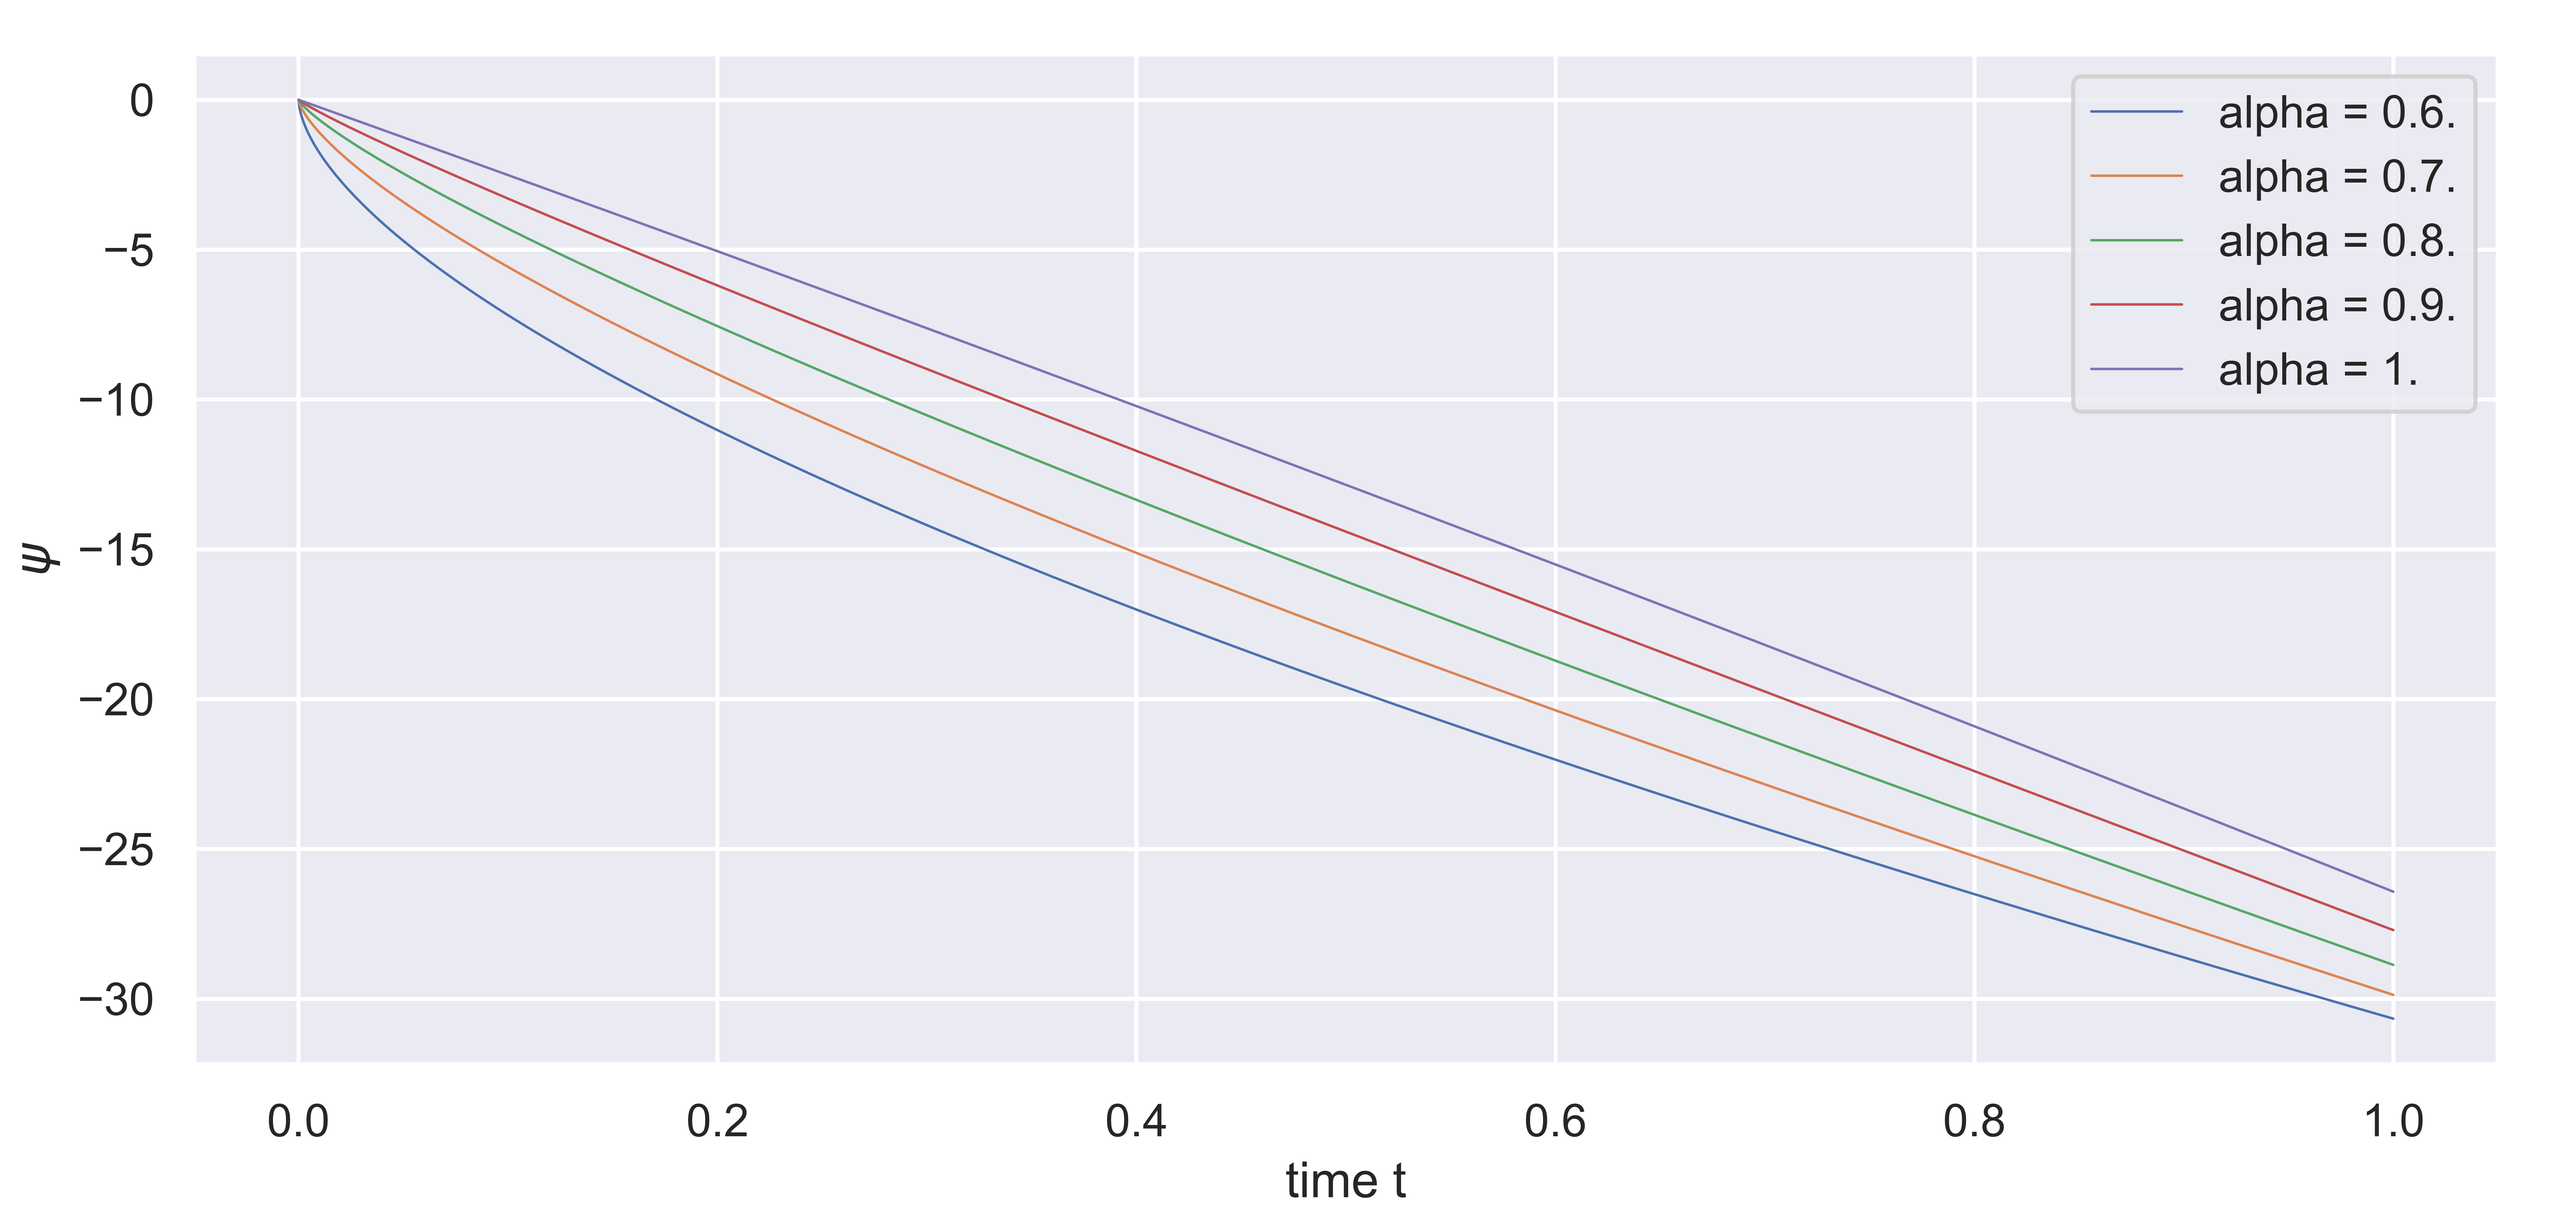
\includegraphics[width = 0.7 \textwidth]{../addition_part/images/numerical_studies/1a.png}
\caption{Plot of $\psi$, which is a key element for the computation of the optimal strategy in \cite{HanWong}. }
\label{fig:1A}
\end{figure}



\begin{figure}
\centering
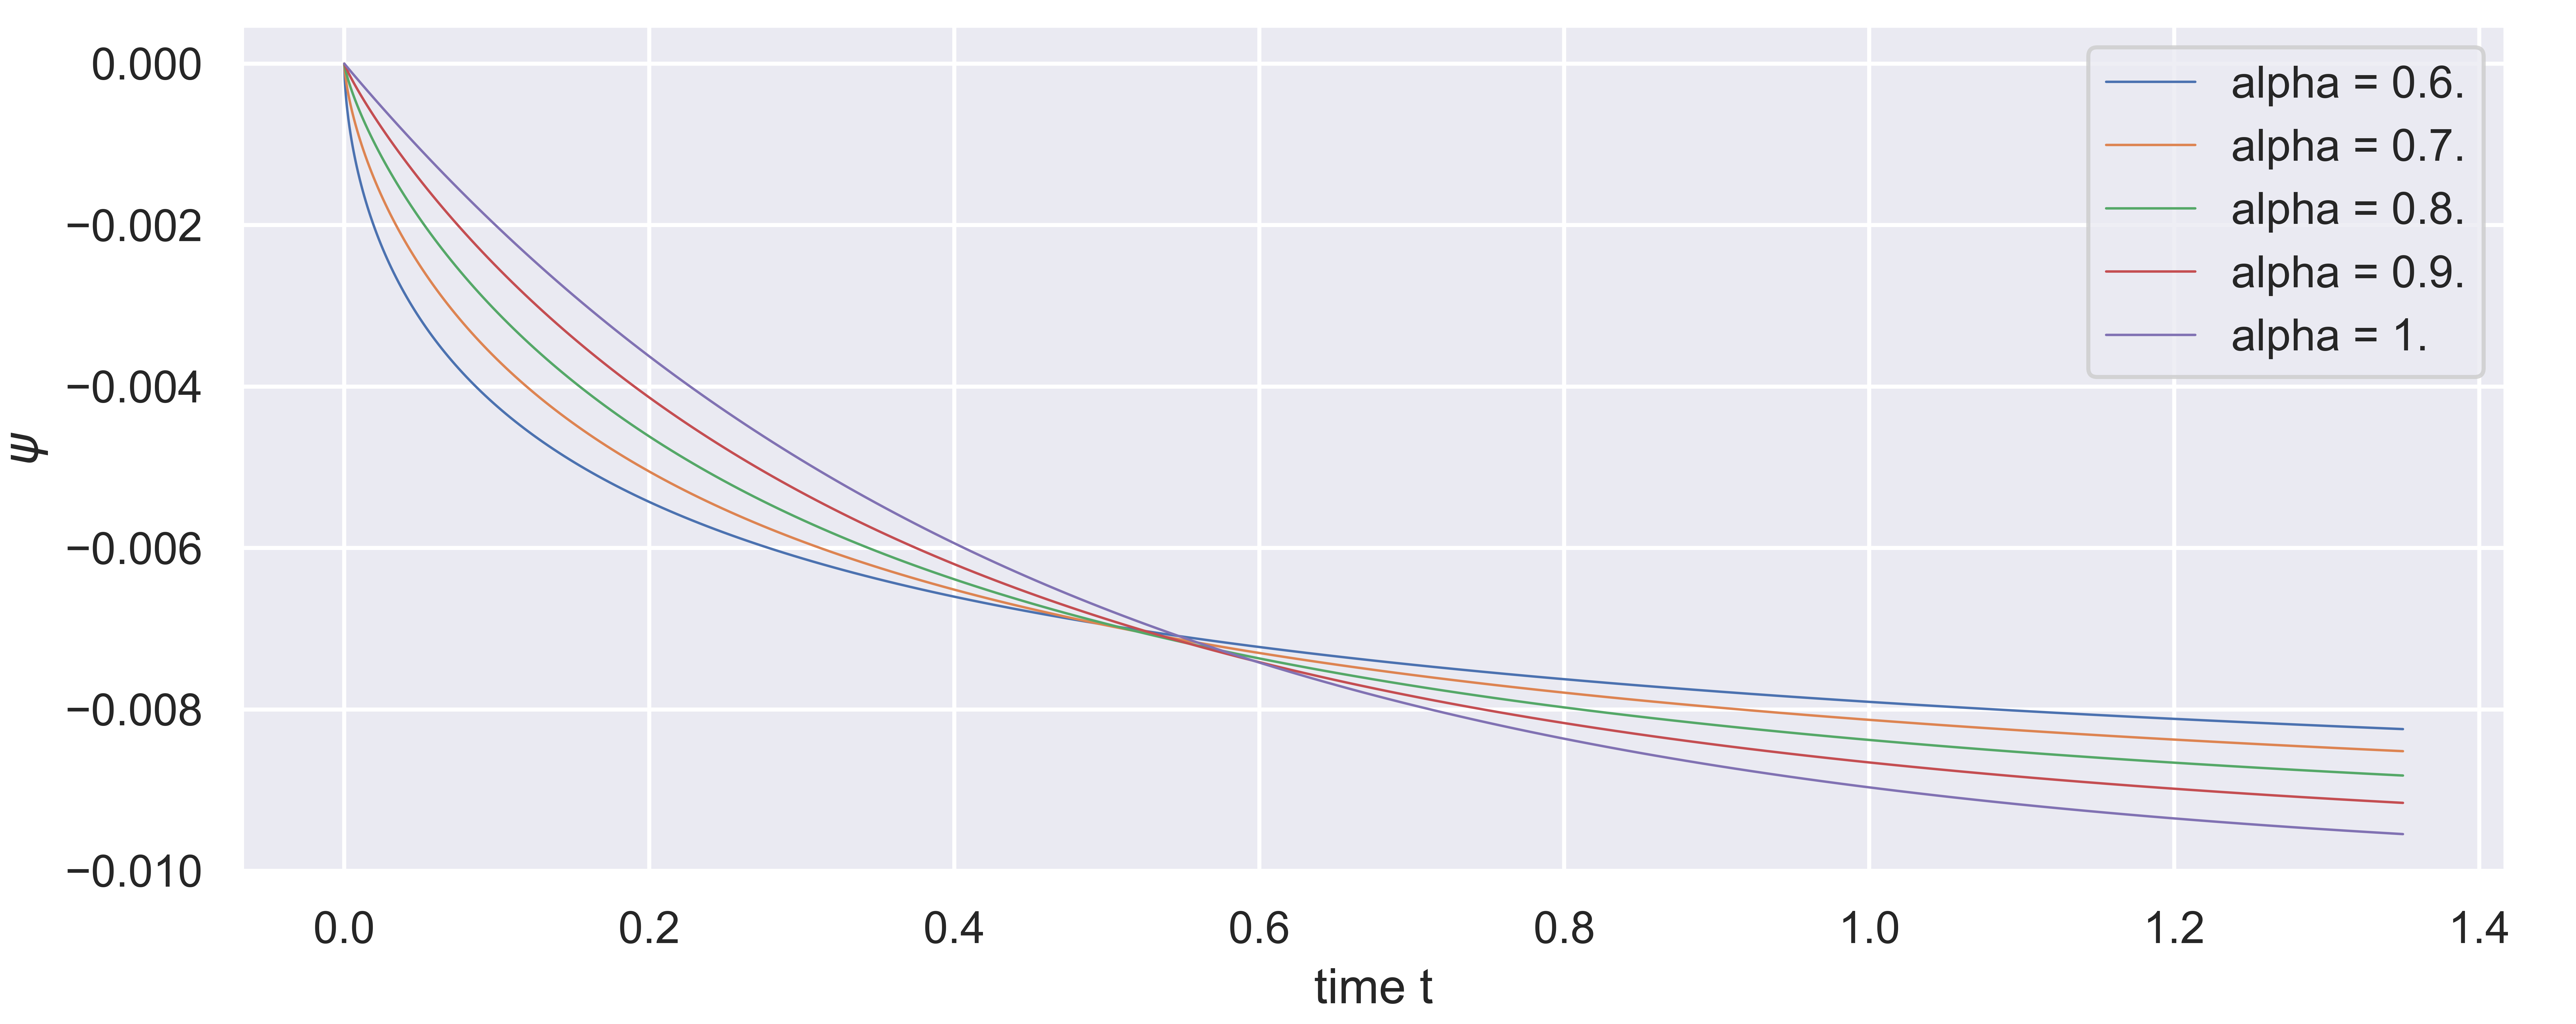
\includegraphics[width = 0.7 \textwidth]{../addition_part/images/numerical_studies/1b.png}
\caption{Plot of $\psi$, under another set of coefficients. }
\label{fig:1B}
\end{figure}









Then, the following step in our research could be computing the optimal strategy, $u^*_t$. To begin with, Han and Wong in \cite{HanWong} fix the volatility and the wealth in the process. As a result, we don't need to simulate anything yet, all the quantities are deterministic. On the other hand, following the definition of $u^*$ (eq. (\ref{eq:optimal_solution})), one sees  that the optimal strategy is heavily dependent on $\psi$ through $A_t$ (eq. (\ref{eq:At})). 
The computations for different alphas can be seen on the fig. \ref{fig:2A} and fig. \ref{fig:2B}, under two sets of parameters given in table \ref{tab:coef2}. Until now, we indeed found the same plots as in \cite{HanWong}, confirming the observations they jotted down in the paper.

\begin{table}
\begin{center}
\begin{tabular}{   m{4.5 cm} | m{4.5 cm} | m{4.5 cm}   } 
\hline
 Parameters & Graph \ref{fig:2A} & Graph \ref{fig:2B} \\ 
\hline
\hline
$\sigma$ & $0.04$ & $3$ \\
\hline
$V_0$ & $0.5$ & $0.5$ \\
\hline
$V_t$ & 0.5 & 0.5 \\
\hline
$x_0$ & $1$ & $1$ \\
\hline
$X_t^*$ & 1 & 1 \\
\hline
$r$ & $0.01$ & $0.01$ \\
\hline
$\rho$ &$ -0.56$ &  $-0.56$\\
\hline
$\theta$  &  $0.15$ &$ 0.15$ \\
\hline
$\kappa$ & $2.25$ & $2.25$ \\
\hline
$\phi$ & $0.15$ &  $0.15$ \\
\hline
T & 1.35 & 1.35 \\
\hline

\end{tabular}
\caption{The two different sets of parameters for $u^*$.}
\label{tab:coef2}
\end{center}
\end{table}



\begin{figure}
\centering
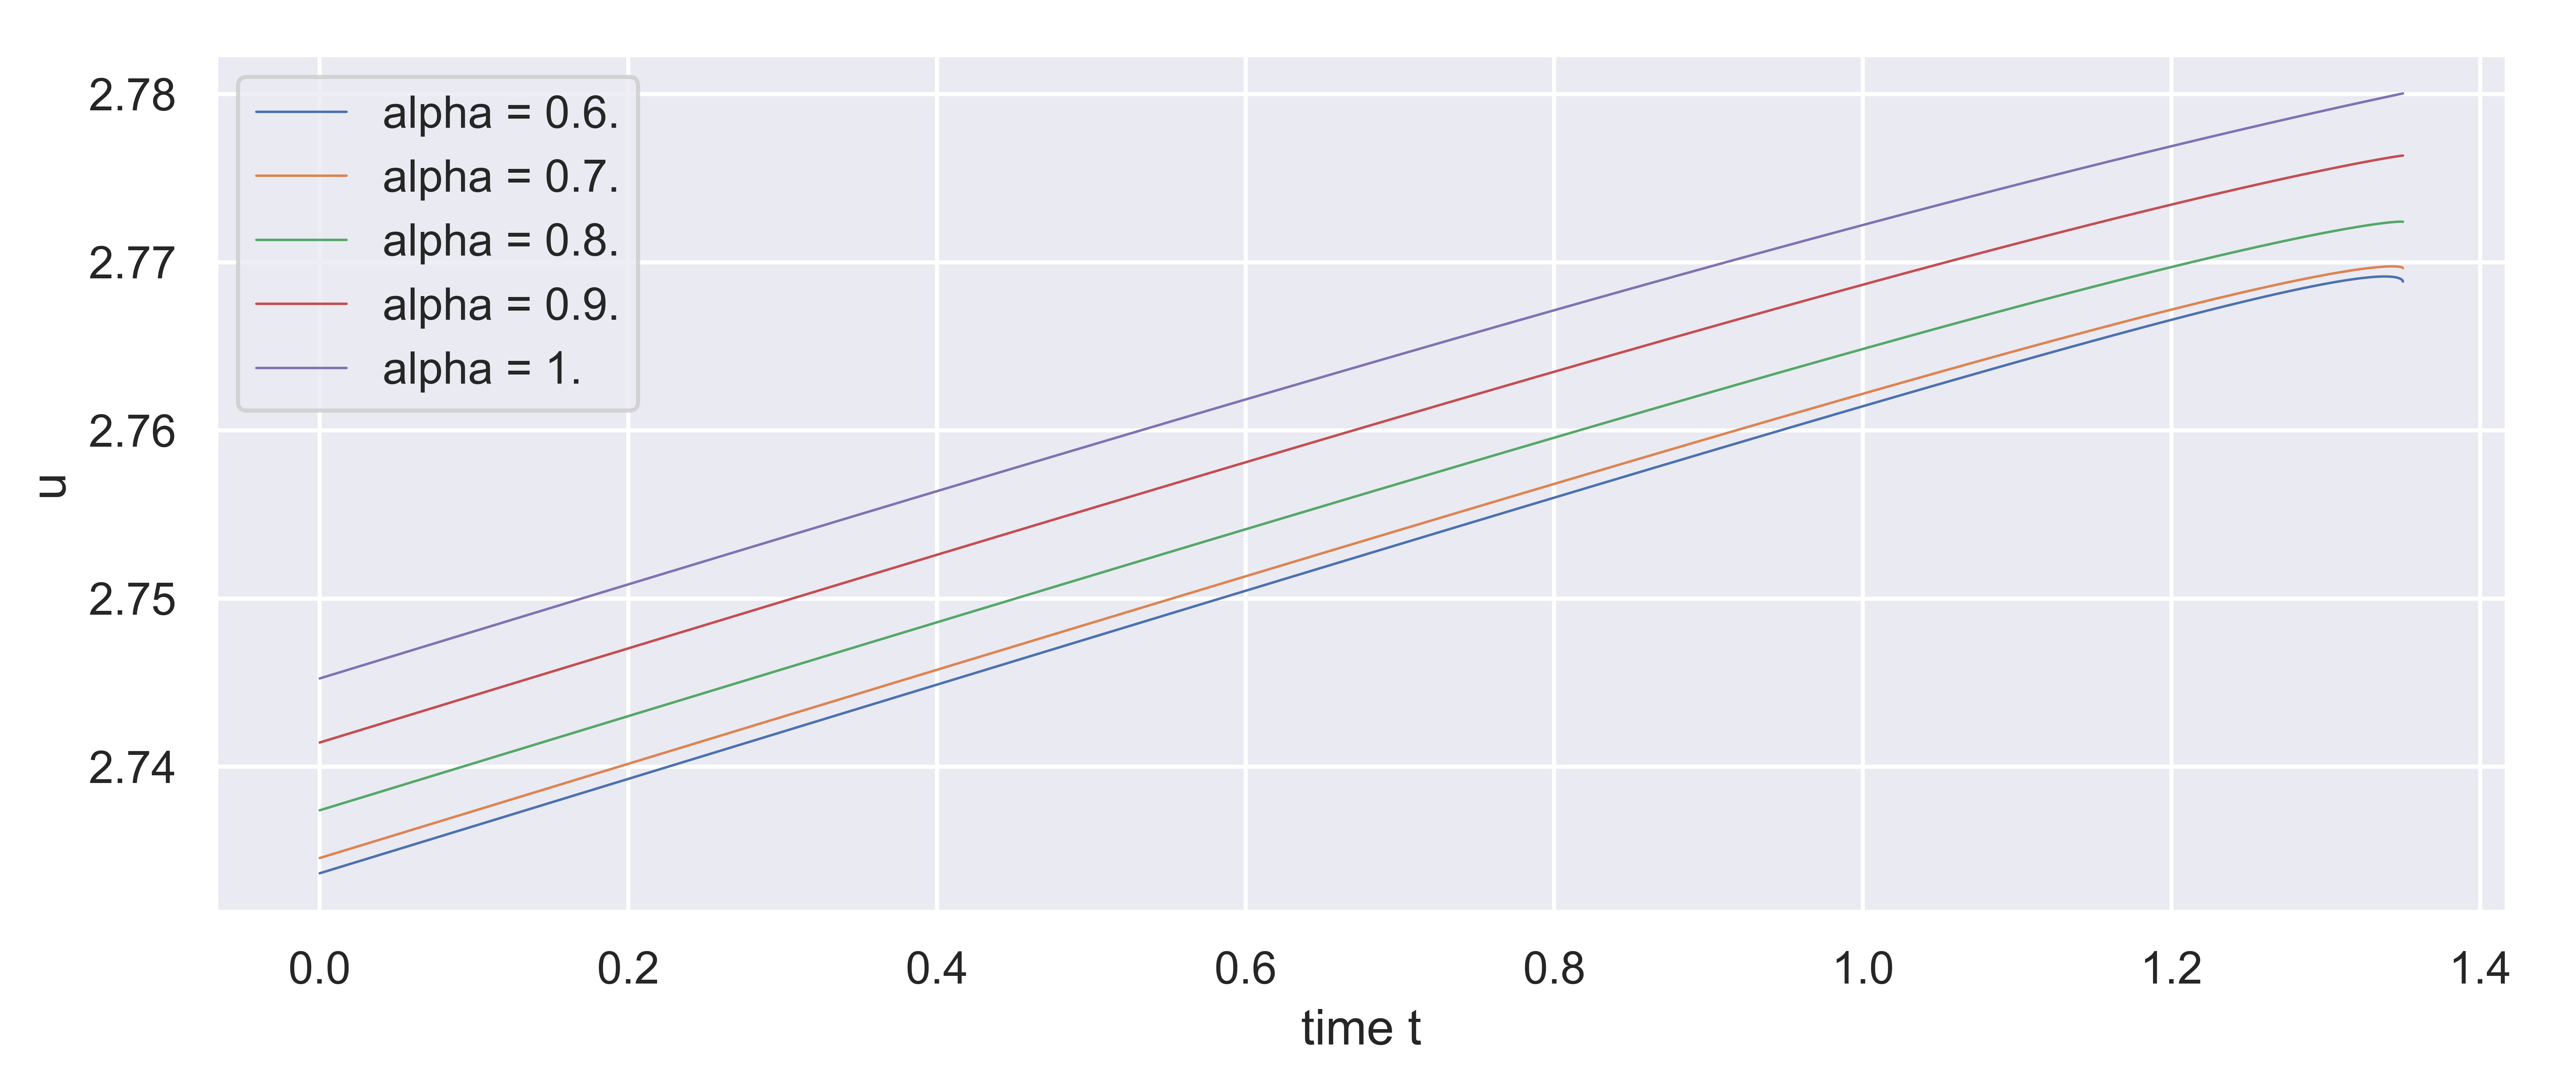
\includegraphics[width = 0.7 \textwidth]{../addition_part/images/numerical_studies/2a.png}
\caption{Optimal strategy, first set of parameters, fixed volatility and wealth.}
\label{fig:2A}
\end{figure}

\begin{figure}
\centering
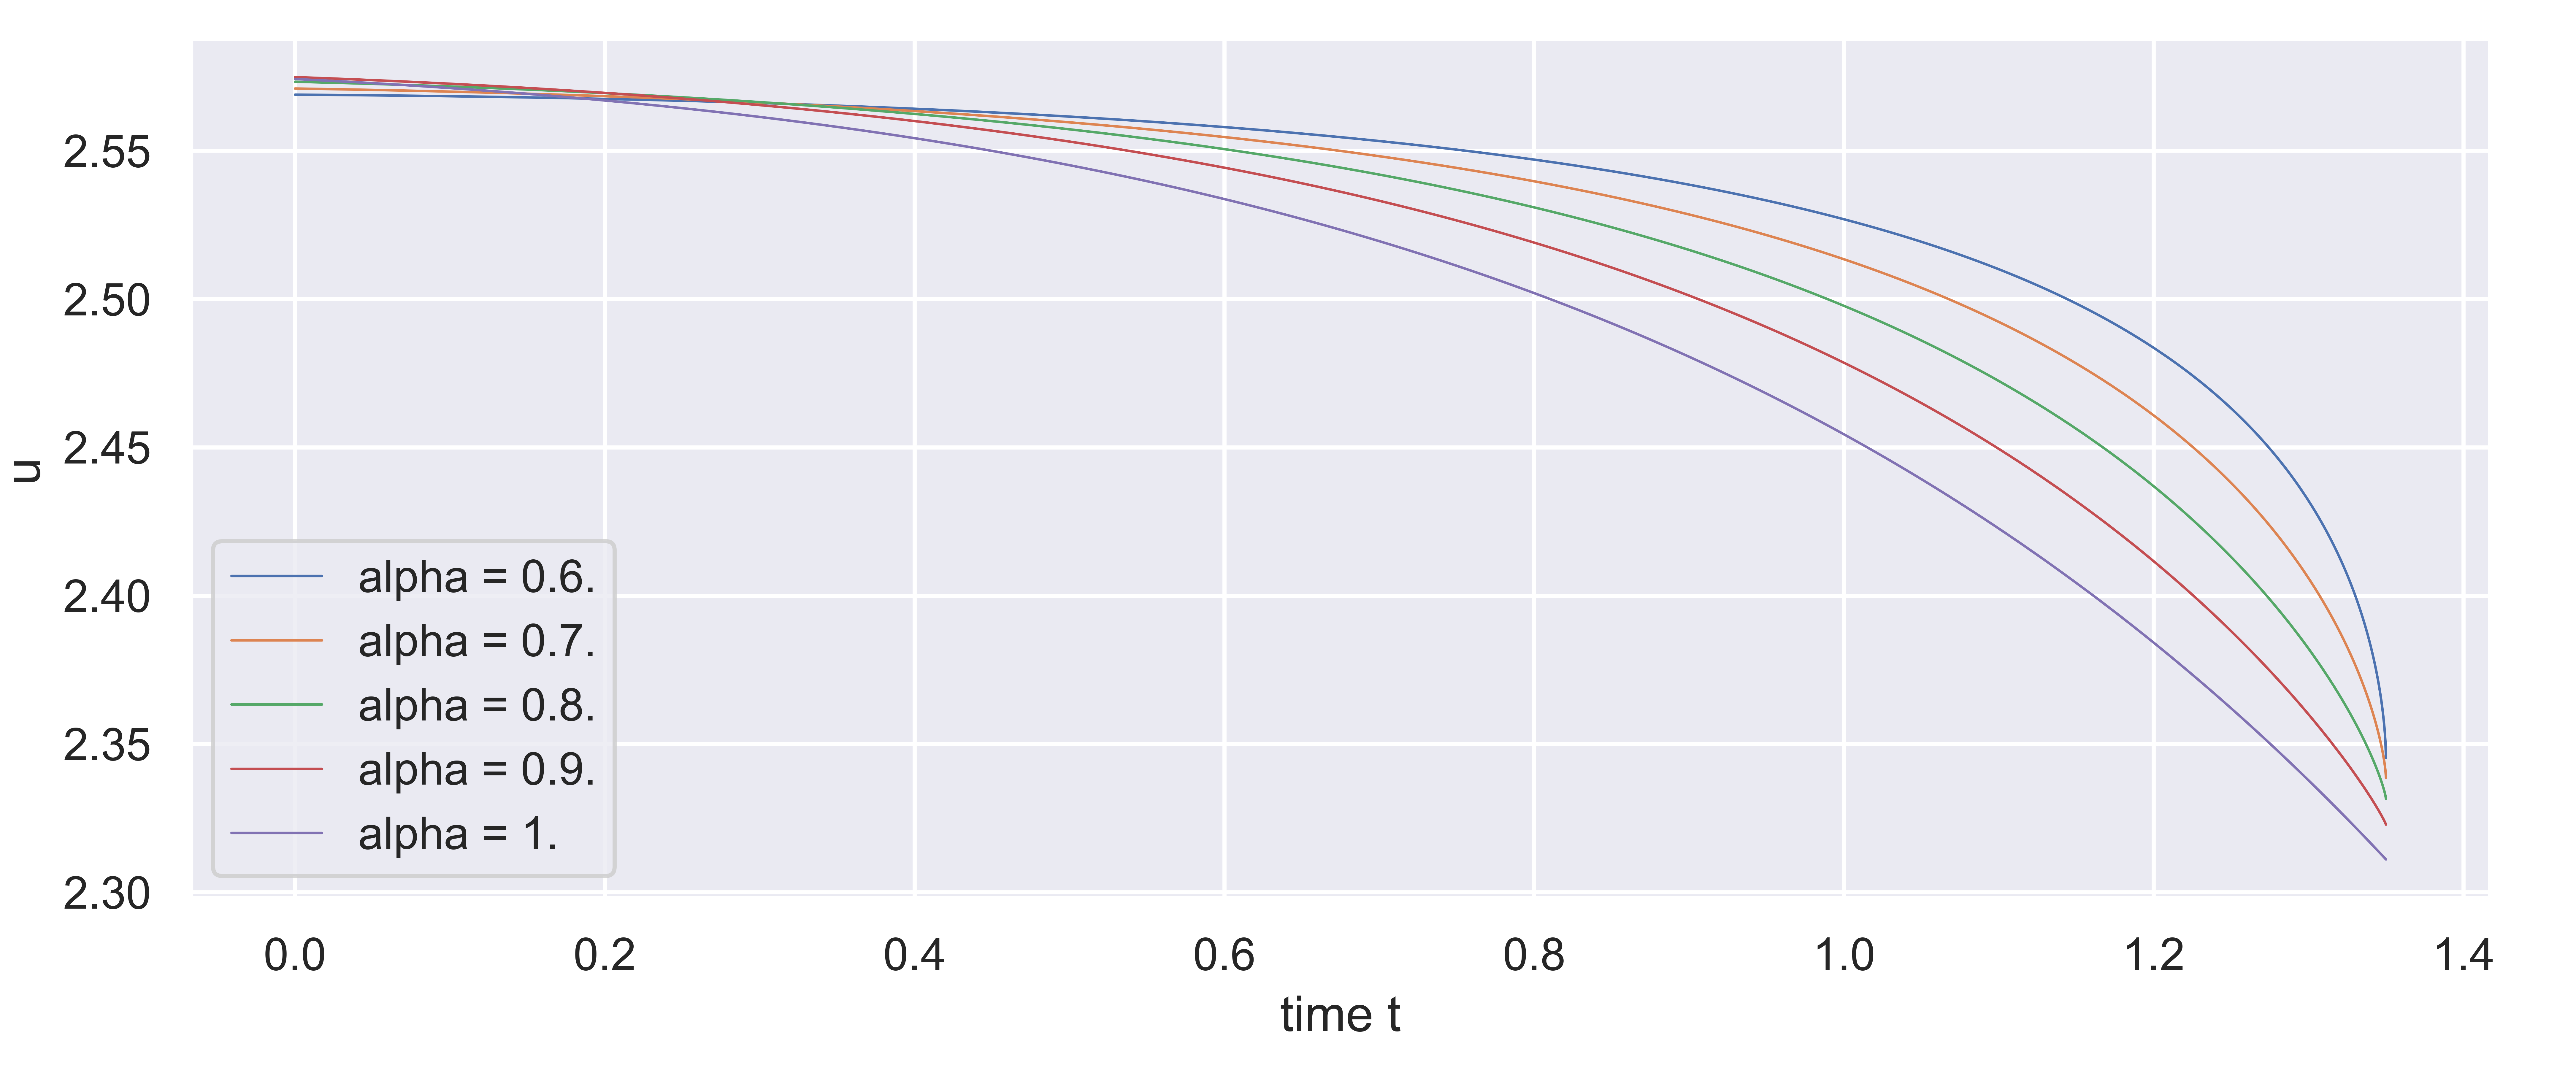
\includegraphics[width = 0.7 \textwidth]{../addition_part/images/numerical_studies/2b.png}
\caption{Optimal strategy, second set of parameters, fixed volatility and wealth.}
\label{fig:2B}
\end{figure}

































\section{Simulating Variance and other stochastic Processes }
\label{processes}

\subsection{Method for simulation}

In order to add some randomness to the model, we need to simulate stochastic processes (i.e. random processes). This is done by integrating random variables into the equations\footnote{In our case, we simulate normal random variables that appear through the Brownian motion of the equations.}.

The easiest case to simulate is the markovian one. Its simplicity comes from the possible conversion between the integral expression and the differential form / flow form. 
An equation that look like this:


$$
d V_t = \kappa  (  \phi - V_t ) dt + \sigma \sqrt{V_t} dB_t 
$$

can be approximated, over a discrete time-grid by this discrete equation:

$$
V_{t+\Delta t} - V_t = \kappa  ( \phi - V_t ) \Delta t + \sigma \sqrt{V_t} \mathcal N ( 0, \Delta t )  
$$

where $\mathcal N ( 0, \Delta t )  $ coins a normal random variable with mean $0$ and variance $\Delta t $. Recall also that 
$$  \mathcal N ( 0, \Delta t )  = \sqrt{ \Delta t } \mathcal N ( 0, 1 )   $$

The good part of this expression is that it does not depend on the discretization of the times since Brownian motion has independent increments. Thus, one can lower the number of points of that expression without affecting the precision of the rest of the computations. 

Here we apply that idea of discretization to our main equations :

\begin{align}
V_{t+\Delta t}  &= V_t + \kappa  ( \phi - V_t ) \Delta t + \sigma \sqrt{V_t} \mathcal M  \\
\mathcal M &= \rho  \left ( \mathcal N_1 ( 0, \Delta t )  + 2 \theta \sqrt{ V_t} \Delta t \right ) +   \sqrt{ 1 - \rho^2 } \mathcal N_2 ( 0, \Delta t ) \\
S_{t+\Delta t} &= S_t + S_t ( r_t + \theta V_t ) \Delta t + S_t \sqrt{V_t} \mathcal N_1 ( 0, \Delta t ) , \quad S_0 > 0 
\end{align}

Please note that if a process can not be expressed as a flow, then one can not simulate the process in such a way. The non-markovian cases we deal with are the rough cases, and other methods are presented in section \ref{rough_heston}.

At this stage, we are able to simulate all the processes from the equations we describe at the beginning of the chapter. However, a problem arises: a Brownian motion can be negative and lead the expression towards negative values, while one still needs to take the square root of the volatility in the dynamics. 

\subsection{How to deal with negative variance ?}

Following the advices from \cite{reflexion}, one is able to deal with negative variance. Since variance is simulated with the help of a Brownian motion, for certain sets of parameters, it reaches zero with positive probability (actually, one condition assures us that the variance will be negative with probability 0, cf. Feller Condition in appendix \ref{feller_condition}). However, the variation process is taken under a square root, making it problematic when the process crosses the x-axis. At the same time, changing the equations by forcing the variance to remain positive may have an impact on the simulation. We want to minimize the latter.

In \cite{reflexion}, Roger Lord, Remmert Koekkoek and Dick van Dijk propose to include three functions in the variance process. The variance becomes:

\begin{align*}
\widetilde{V}(t + \Delta t) &= f_1( \widetilde{V} (t) ) - \kappa \Delta t \cdot \left ( f_2( \widetilde{V}(t) ) - \overline{V} \right ) + \omega  f_3( \widetilde{ V} (t) )^\alpha \Delta W_V(t) \\
V(t+\Delta t ) &= f_3 ( \widetilde{V}(t + \Delta t) ) 
\end{align*}

where $\widetilde{V}$ is a process that might be negative, $ \overline{V}$ the long-term variance.


\begin{table}
\begin{center}
\begin{tabular}{  | m{3 cm} | m{1.5 cm} | m{1.5 cm} | m{1.5 cm} | } 
\hline
Scheme & $f_1$ & $f_2$ & $f_3$  \\ 
\hline
\hline
Absorption & $  x^+ $ & $ x^+ $ & $ x^+ $ \\
\hline
Reflection & $ \abs x $ & $ \abs x $ & $ \abs x $ \\
\hline
Full truncation & $ x $ & $ x^+ $  & $ x^+ $ \\
\hline

\end{tabular}
\caption{Three different schemes, $x^+ = \Max(0,x) $.}
\label{tab:reflections}
\end{center}
\end{table}

The whole discussion of the paper is the attempt to improve the classical "reflection" method used (cf. table \ref{tab:reflections}). We omit the details; they prove in the paper strong convergence of full truncation, so this is the scheme we are going to use for the simulations. For shortness, we haven't written all the proposed schemes and justification. One is invited to take a look at the original paper. Their main concern was to keep the bias induced by the choice of the function to be the smallest.












\subsection{Results of simulations}

The previous sections explained the technical difficulties of simulating stochastic volatility models, when the model is markovian. In the following page, one is able to see the different computations and simulations, gears of the whole mechanism (fig. \ref{fig:dynamics}). I couldn't find the parameters used in \cite{HanWong}, so I used the set of coefficients given by table \ref{tab:coef3}. The plots are not very informative, though they are a proof of the fact that my computations are running. We observe the impact of randomness on the model. One can in particular compare the graph of $u^*$ when no randomness is involved to the new ones. We clearly see how $u*$ is affected by the incorporated Brownian motion. Also, one can notice on the plot of the volatility the effect of negative variance on the process. The full truncation makes the volatility equal to 0 on certain portion of the time.

At this stage, it is also possible to draw the efficient frontier which puts into relation the expected payoff with the risk he has to take. We take eq. (\ref{eq:variance_process}) and compute it for various $\alpha$ and various $c$. The former has an impact on $\psi$, and the latter appears in the expression of the variance.  Then we get the frontier, which shows the impact of the model over the mean-variance portfolio selection. The figure for the efficient frontier is fig. \ref{fig:efficientfrontier}, using the same parameters as in the previous paragraph. We observe that there is a (negative) linear relationship between $\alpha$ and the payoff, which indicates that a rougher model forecasts more payoff in average for a given level of risk. Also, one can observe the classical relationship between the payoff and the variance, for $\alpha = 1$.



\begin{figure}
\centering


\subfloat{{
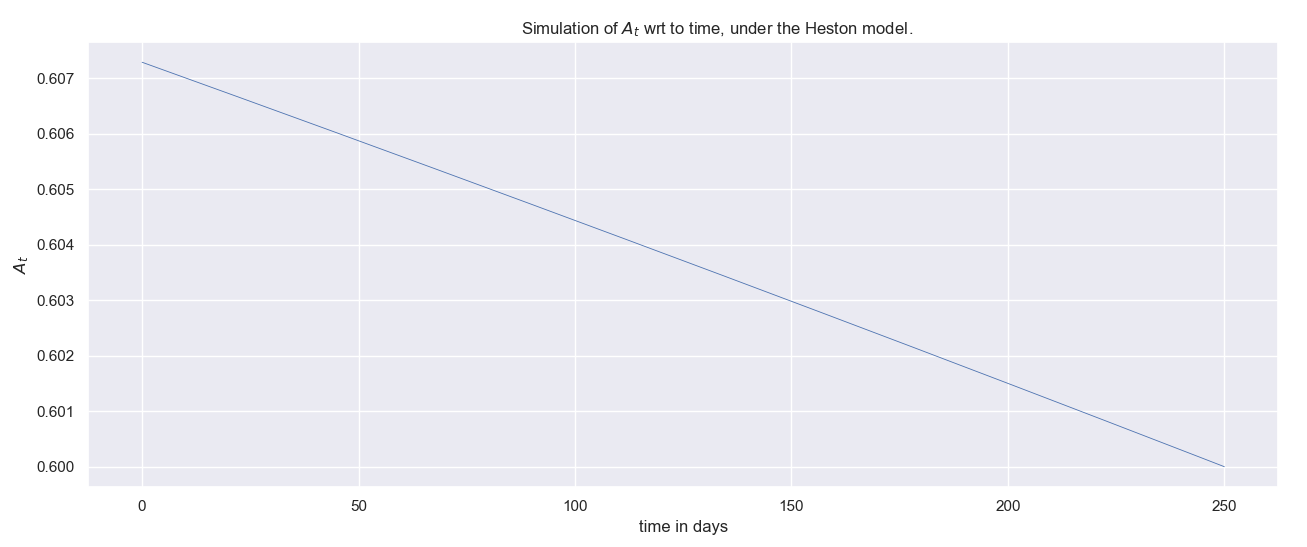
\includegraphics[width = 0.48 \textwidth]{../addition_part/images/numerical_studies/3A_t.png}
}}
\subfloat{{
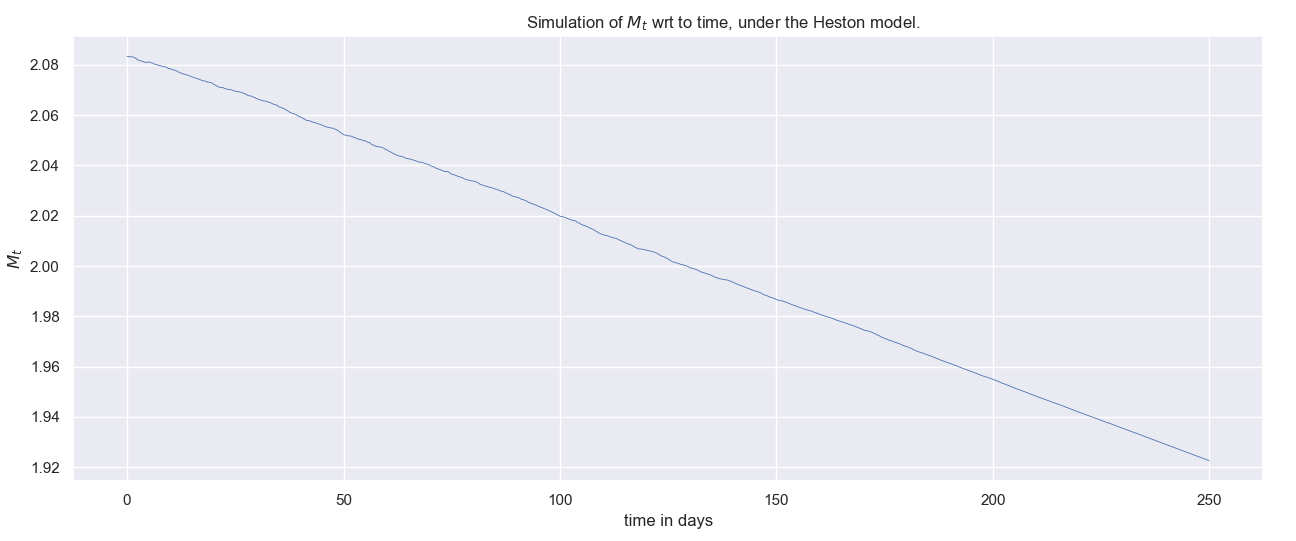
\includegraphics[width = 0.48 \textwidth]{../addition_part/images/numerical_studies/3M_t.png}
}}\\
\subfloat{{
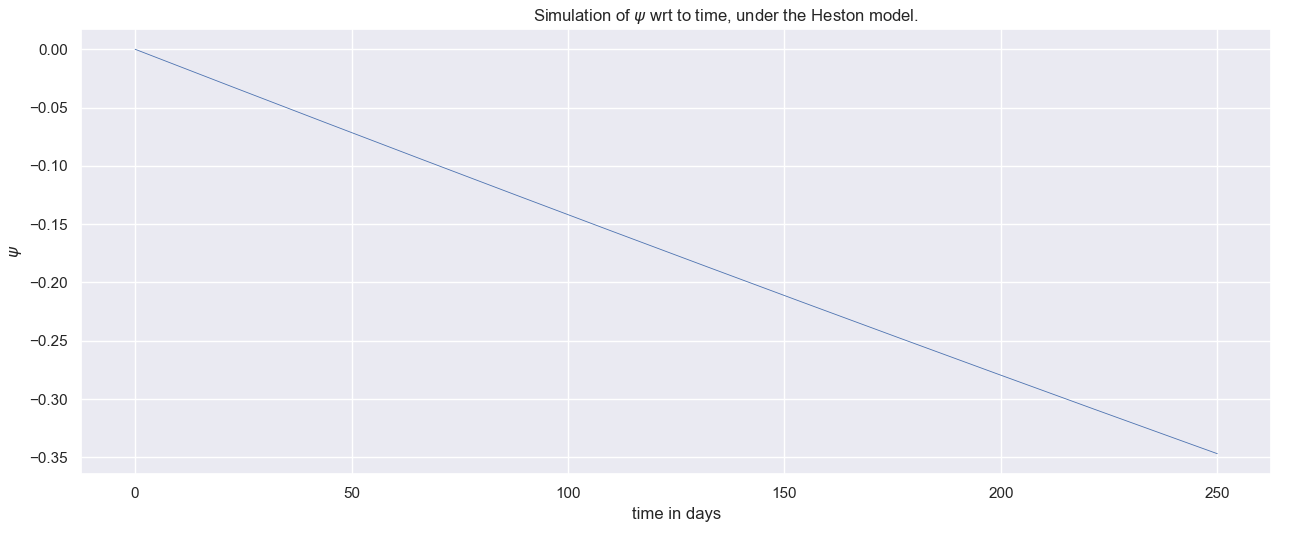
\includegraphics[width = 0.48 \textwidth]{../addition_part/images/numerical_studies/3psi.png}
}} 
\subfloat{{
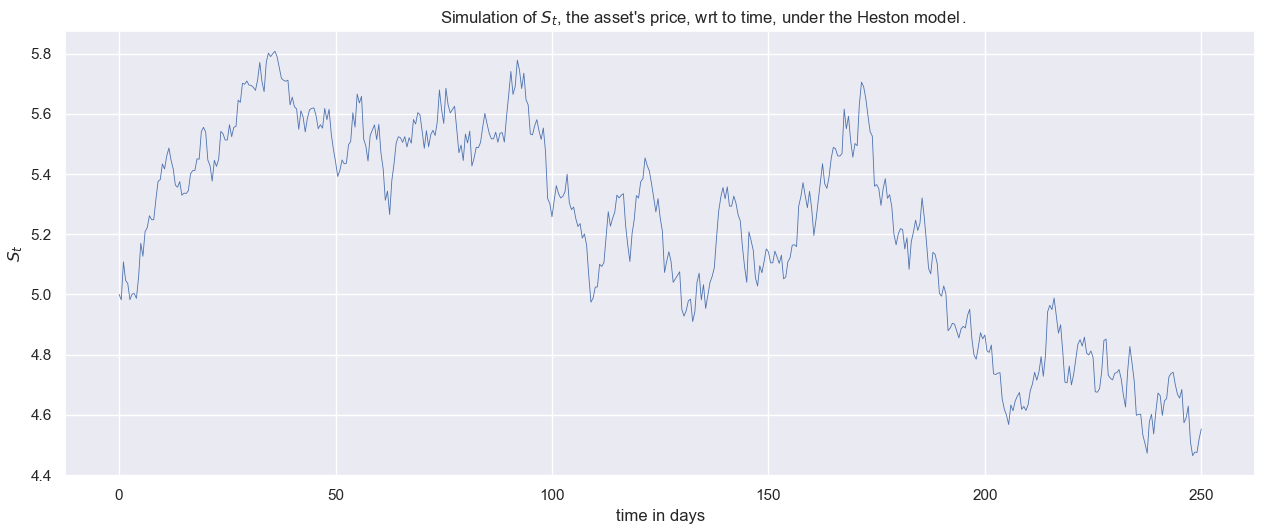
\includegraphics[width = 0.48 \textwidth]{../addition_part/images/numerical_studies/3S_t.png}
}}\\
\subfloat{{
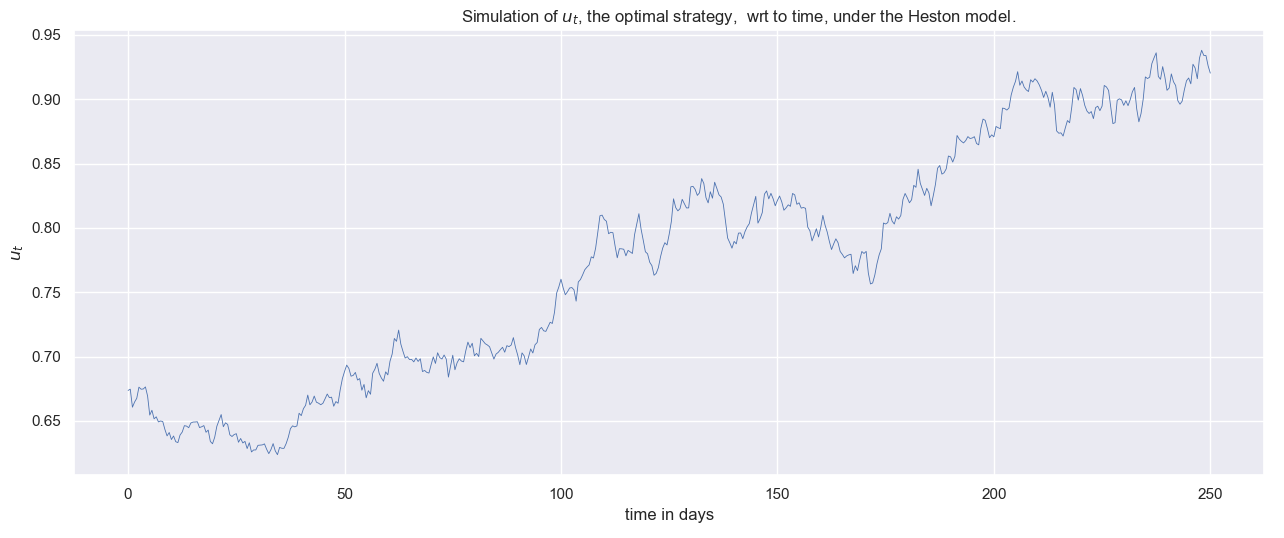
\includegraphics[width = 0.48 \textwidth]{../addition_part/images/numerical_studies/3u_t.png}
}} 
\subfloat{{
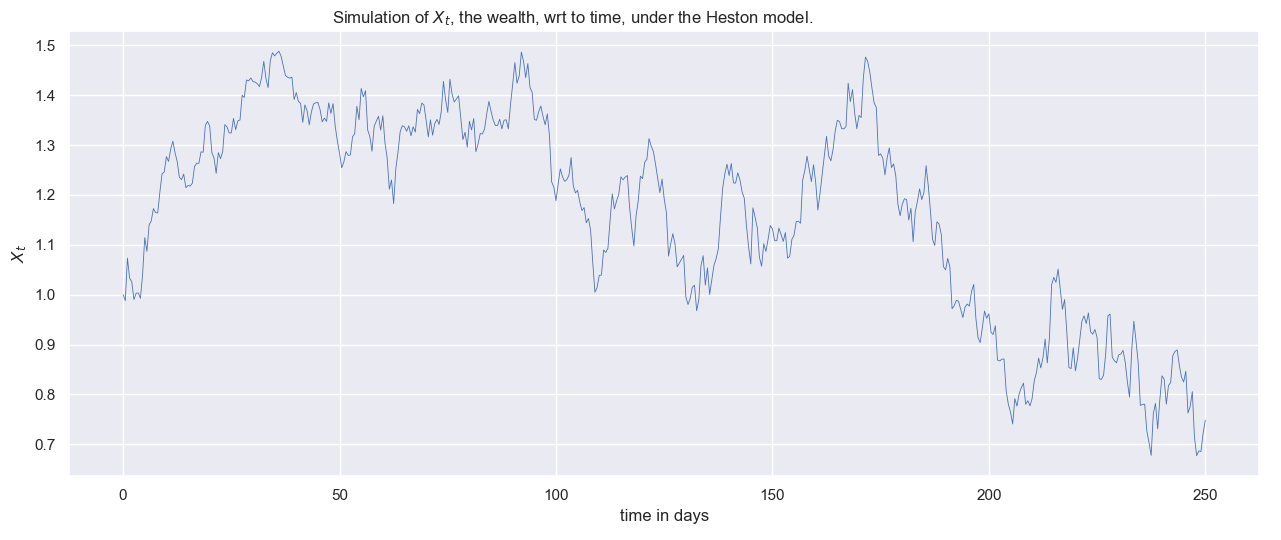
\includegraphics[width = 0.48 \textwidth]{../addition_part/images/numerical_studies/3X_t.png}
}}\\
\subfloat{{
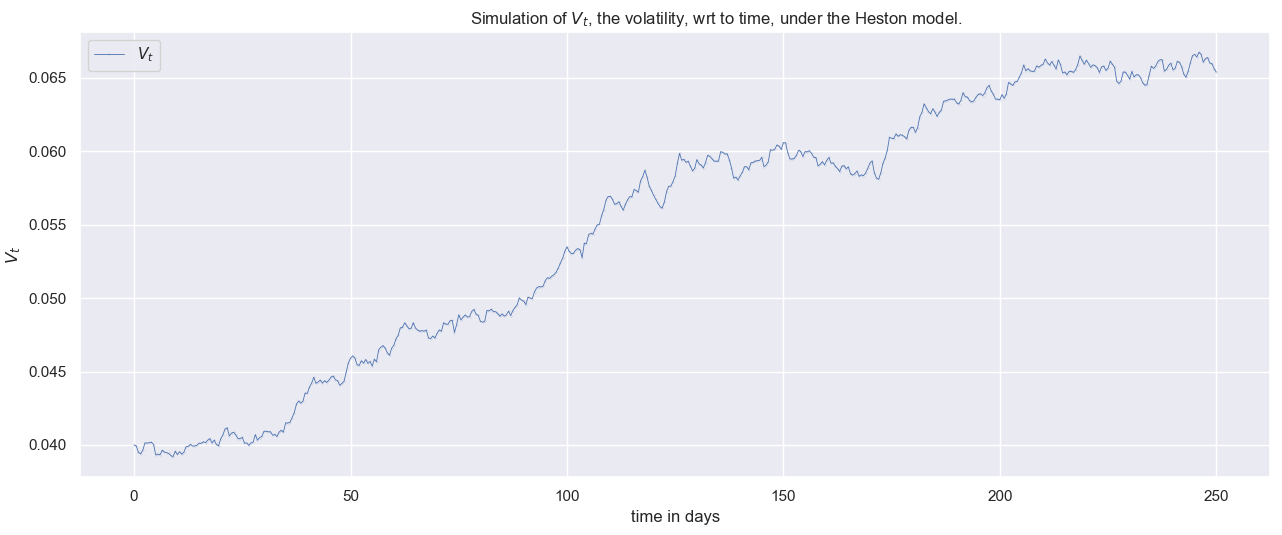
\includegraphics[width =  0.5 \textwidth]{../addition_part/images/numerical_studies/3V_t.png}
}} 

\caption{Dynamics of the different processes and strategies. Respectively, from left to right, top to bottom, $A_t$, $M_t$, $\psi$, $S_t$, $u_t$, $X_t$, $V_t$.}
\label{fig:dynamics}
\end{figure}









\begin{table}
\begin{center}
\begin{tabular}{   m{4.5 cm} | m{4.5 cm}   } 
\hline
 Parameters & Plots  \ref{fig:dynamics} and \ref{fig:efficientfrontier}  \\ 
\hline
\hline
$\sigma$ & 0.03  \\
\hline
$V_0$ &  0.04 \\
\hline
$x_0$ &  1 \\
\hline
$S_0$ & 1 \\
\hline
$r$ & 0.03 \\
\hline
$\rho$ & -0.7\\
\hline
$\theta$  & 0.6  \\
\hline
$\kappa$ & 0.1 \\
\hline
$\phi$ & 0.3  \\
\hline
T & 1 \\
\hline
\end{tabular}
\caption{Set of parameters for simulations of the processes and of the efficient frontier.}
\label{tab:coef3}
\end{center}
\end{table}







\begin{figure}
\centering
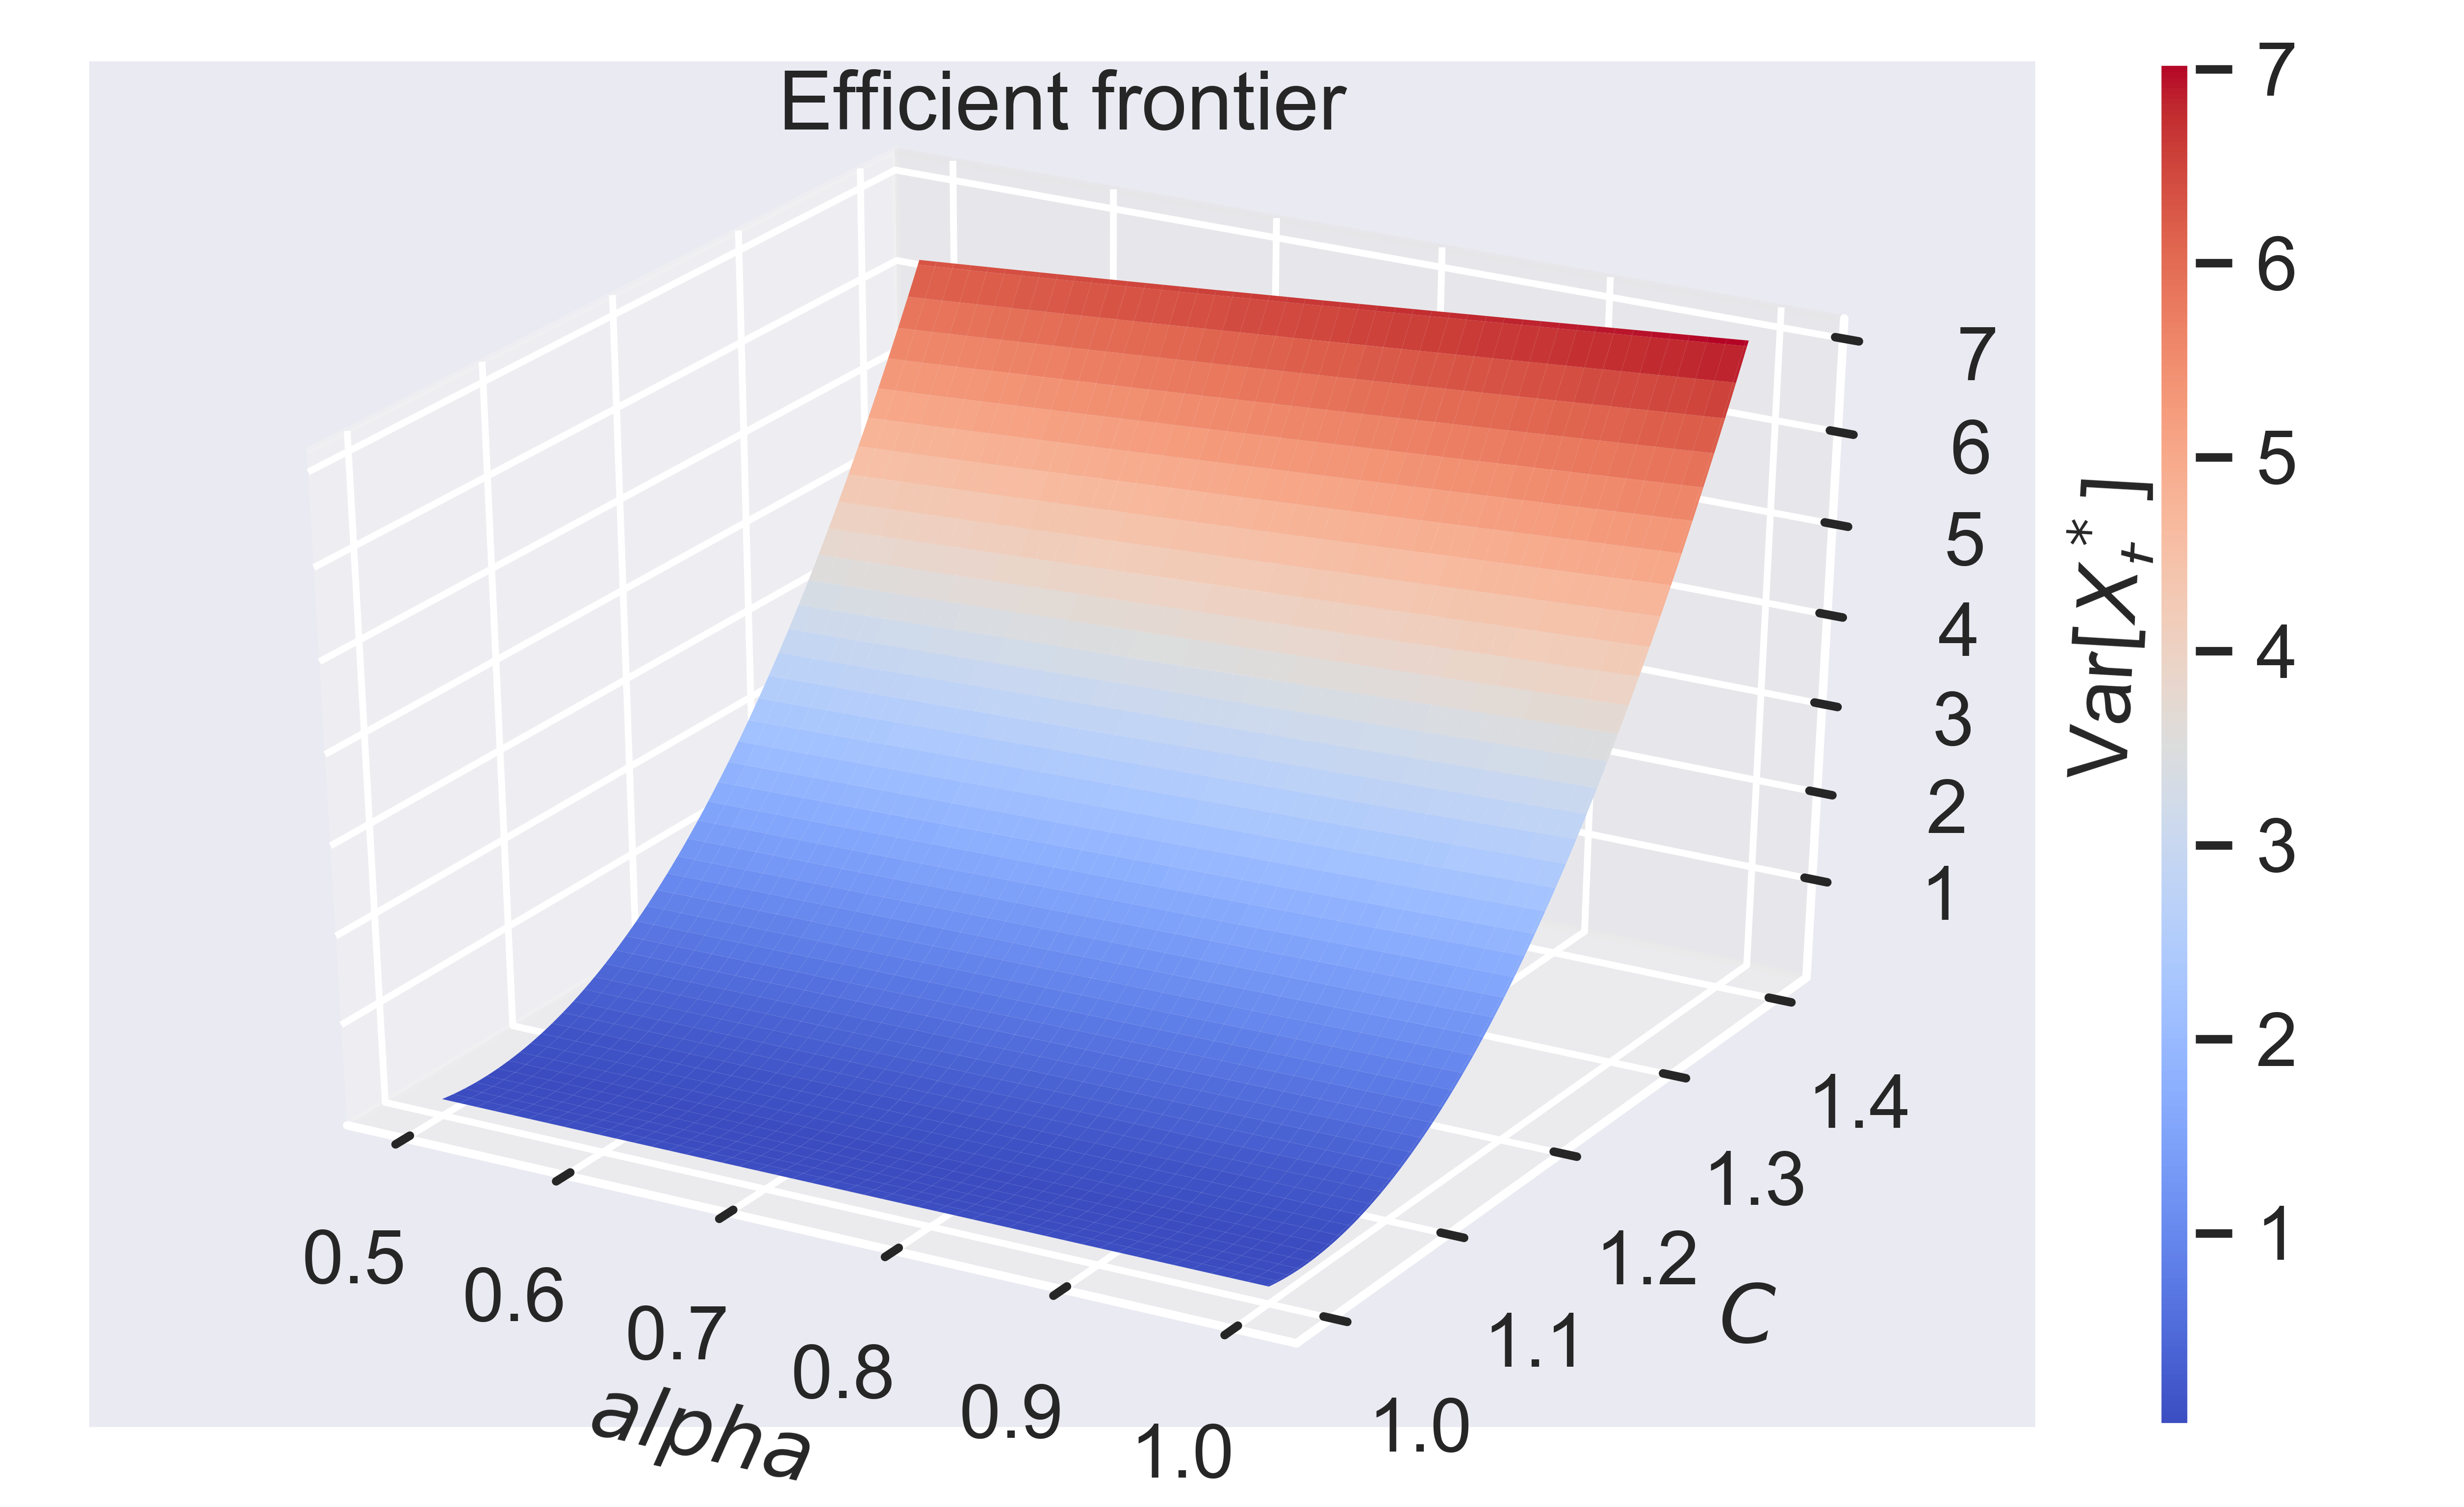
\includegraphics[width = 0.5 \textwidth]{../addition_part/images/numerical_studies/efficient_frontier.png}
\caption{Efficient frontier where one see the influence of $\alpha$ and the choice of the target wealth upon the variance of the portfolio.}
\label{fig:efficientfrontier}
\end{figure}














\section{Rougher Path for Heston }
\label{rough_heston}
As mentioned in \cite{HanWong}, markets are better described by processes that include roughness, or in other words some memory. We describe here two ways to simulate a rougher path. That way, we will be able to simulate the expectation of the wealth as they did in the paper by MonteCarlo method, and compare that indeed, a rougher model leads to a solution closer to the true value.

\subsection{Lifted Heston}

In the paper \cite{lifted}, an attempt to generate rougher path with the help of non-rough path is proposed. Abi Jaber's idea is to use a Heston model with $n$ multi-factors, sharing the same Brownian motion but mean reverting at different speeds. The advantage of the lifted Heston is sharing the best properties of roughness and classic Heston : it is at the same time markovian, a semimartingale, allows a characteristic function and is computed faster than rough Heston.

In more detail, the advantages of that method are, as written in the paper:

\begin{itemize}
\item reproduces the same volatility surface as the rough Heston model for maturities ranging from one week to two years,
\item mimics the explosion of the at-the-money skew for short maturities,
\item calibrates twenty times faster than its rough counterpart,
\item is easier to simulate than the rough model.
\end{itemize}

First, recall the equations of the process, under $\alpha = 1$:

\begin{align*}
dV_t &= ( \kappa \phi - \lambda V_t ) dt + \sigma \sqrt{V_t} d \widetilde{B_t}   \\
d \widetilde{B_s } &:= \rho d [ W_{1,s} + 2 \theta \int_0^s \sqrt{ V_u } du ] + \sqrt{ 1 - \rho^2 } d W_{2,s}   \\
d S_t &= S_t ( r_t + \theta V_t ) dt + S_t \sqrt{V_t} d W_{1,t}, \quad S_0 > 0 
\end{align*}

Then, following the method proposed by Abi Jaber in the paper, and adjusting it to take into account that in our case, the risk premium,  $\theta \neq 0$, we then get the following process. The notations for the processes are consistent with the ones from \cite{lifted}, and the constants were adapted to our previous notations:

\begin{align}
d S_t^n &= S_t^n ( r_t + \theta V_t^n ) dt + S_t^n \sqrt{V_t^n} d W_{1,t}, \quad S_0 > 0  \\
dU_t^{n,i} &= \left ( - x_i^n U_t^{n,i} - \lambda V_t^n \right ) dt + \sigma \sqrt{V_t^n}  d \widetilde{B_t}  \label{eq:lifted_1}  \\
d \widetilde{B_s } &:= \rho d [ W_{1,s} + 2 \theta \int_0^s \sqrt{ V_u } du ] + \sqrt{ 1 - \rho^2 } d W_{2,s}   \\
V_t^n &= g_0^n (t) + \sum^n_1 c_i^n U_t^{n,i} \label{eq:lifted_2} \\
g_0^n  \colon t &\to V_0 + \frac{ \kappa \phi} { \lambda } \sum_1^n c_i^n \int_0^t e^{-x_i^n (t-s) } ds \label{eq:lifted_error}
\end{align}

where the $r_i^n, x_i^n, c_i^n$ are defined in the paper p.6, where the $x_i$ and the $c_i$ are functions of $r_i$.

\begin{remarque}
It is written in the paper that one can modify the coefficients $r_i^n$ in order to increase roughness.
\end{remarque}

Actually, I'd like to correct the last equation as it seems to me that there is a typo. I think it should be:

$$ 
g_0^n  \colon t \to V_0 + \kappa \phi \sum_1^n c_i^n \int_0^t e^{-x_i^n (t-s) } ds
$$

The reason why I think it is the case, is because the model doesn't reduce to the classical Heston. As mentioned in the paper, if one takes 
$$ n = 1, \qquad x_i \equiv 0, \qquad c_i \equiv 1 $$

the model shall reduce to the classical Heston. However, one notices that under taking the original equations (\ref{eq:lifted_error}), the variance converges, when $T$ increases, to $\frac {\phi } {\kappa}$ instead of converging to $\phi$ as it should. This can be verified mathematically that under the previously mentioned assumption, the variance process does not come back to the classical case: 


\begin{align*}
V_t^n &= g_0^n (t) + \sum^n_1 c_i^n U_t^{n,i} \\
&= V_0 + \frac{ \kappa \phi} { \lambda } \sum_1^n c_i^n \int_0^t e^{-x_i^n (t-s) } ds 
+ \sum^n_1 c_i^n U_t^{n,i} \\
&= V_0 + \frac{ \kappa \phi} { \lambda } t
+ U_t^{n,1} \\
&= V_0 + \frac{ \kappa \phi} { \lambda } t + U_t^{n,1}
\end{align*}
then 
\begin{align*}
dV_t^n &= \frac{ \kappa \phi} { \lambda } dt + dU_t^{n,1} \\
&=  \frac{ \kappa \phi} { \lambda } dt - \lambda V_t^n dt + \sigma \sqrt{V_t^n}  d \widetilde{B_t} \\
&= ( \frac{ \kappa \phi} { \lambda } - \lambda V_t ) dt + \sigma \sqrt{V_t} d \widetilde{B_t}
\end{align*}

On the other hand, if one takes the other expression of $g_0$, where $\kappa \phi $ substitutes $\frac{ \kappa \phi} { \lambda }$ the results agree with the original variance flow form. I am thus going to stick with that expression of $g_0$ for the simulations.

\begin{figure}
\centering
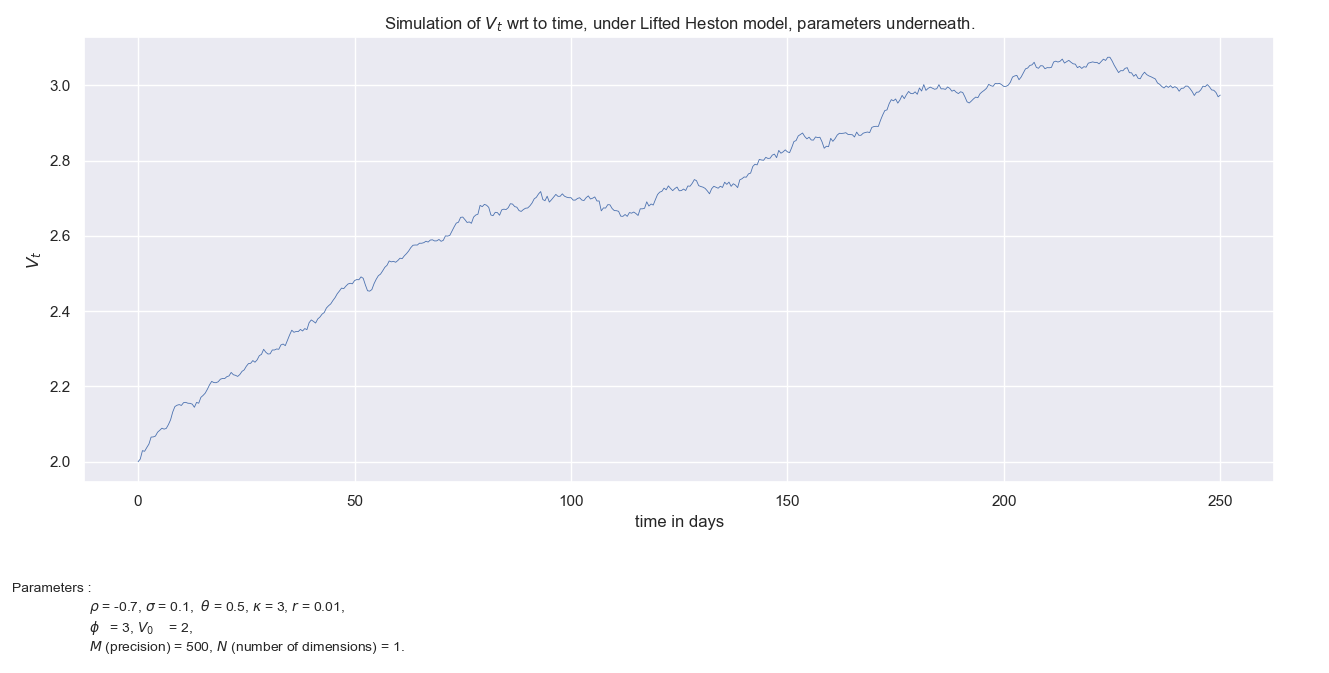
\includegraphics[width = 0.8 \textwidth]{../addition_part/images/numerical_studies/Lifted_V_t.png}
\caption{Lifted Heston as proposed by Abi Jaber in \cite{lifted}, degenerated case into normal Heston.}
\label{fig:liftedV}
\end{figure}

\begin{figure}
\centering
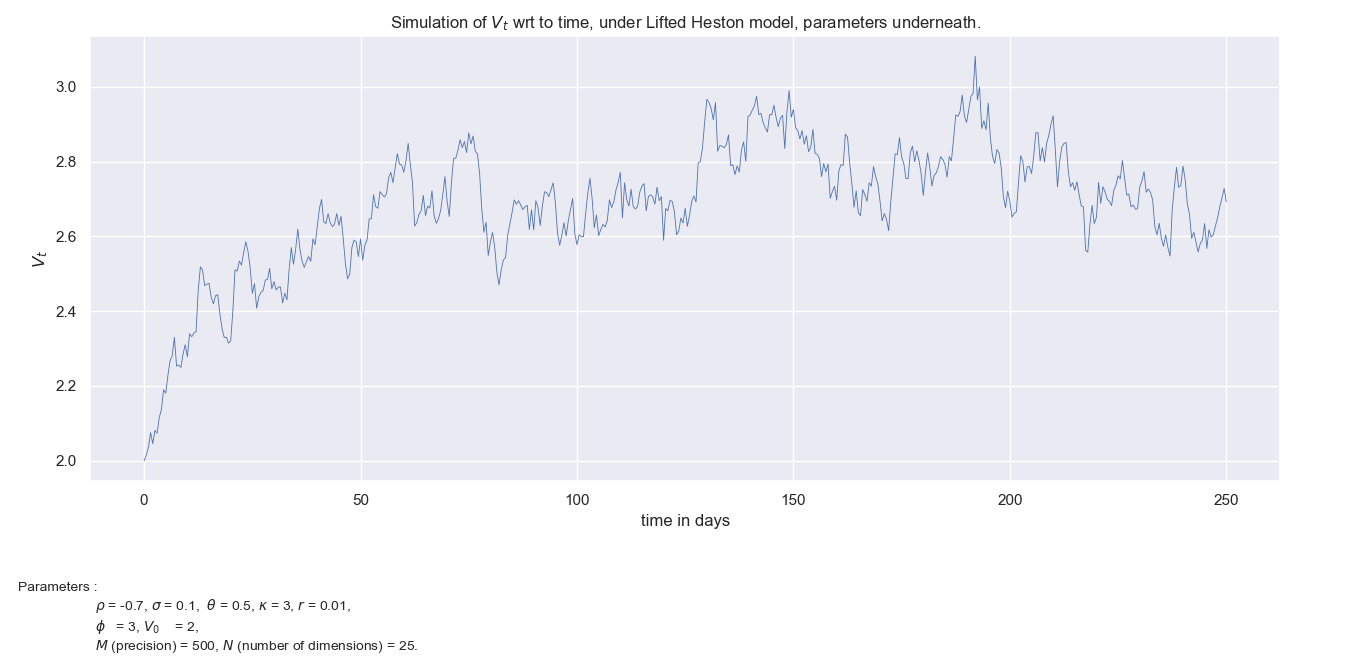
\includegraphics[width = 0.8 \textwidth]{../addition_part/images/numerical_studies/Lifted_V_t_2.png}
\caption{Lifted Heston as proposed by Abi Jaber in \cite{lifted}, 25 dimensions.}
\label{fig:liftedV_2}
\end{figure}



So at the end of the day, in order to compute the lifted Heston, one first computes $g_0^n$, then simulates $\forall i \colon U_t^i$ and $V^n$ incrementally. 

Additionally, aware of the difficulty of dealing with negative variance, I used the same scheme as for normal Heston, in other words the full truncation. The expression of the volatility using the four functions $f_i$ looks like this. Plugged in eq. (\ref{eq:lifted_1}) and in eq. (\ref{eq:lifted_2}):

\begin{align*}
dU_t^{n,i} &= \left ( - x_i^n U_t^{n,i} - \lambda f_2(V_t^n) \right ) dt + \sigma \sqrt{ f_3(V_t^n) }  d \widetilde{B_t} \\
d \widetilde{B_s } &= \rho d [ W_{1,s} + 2 \theta \int_0^s \sqrt{ f_2(V_u) } du ] + \sqrt{ 1 - \rho^2 } d W_{2,s} \\
V_t^n &= f_3 \left ( g_0^n (t) + \sum^n_1 c_i^n U_t^{n,i} \right )
\end{align*}

Also, one can evaluate by hand, before computation, the integral inside $g_0$ :

$$ \int_0^t e^{-x_i^n (t-s) } ds  
= \int_0^t e^{-x_i^n s } ds 
= \begin{cases} 
t, & \mbox{ if } x_i^n = 0 
\\ 
\frac {1} { x_i^n } ( 1 - e^{-x_i^n t } )  , & \mbox{ if } x_i^n \neq 0   
\end{cases}
$$ 

Here are two plots; the first one corresponds to the lifted Heston degenerating to the normal Heston, fig. \ref{fig:liftedV} ; the second plot is the rough Heston generated by 25 dimensional lifted Heston, fig. \ref{fig:liftedV_2}. The first plot shows a variance that is quite similar to the original one (from \ref{fig:dynamics}), and converges to the long term expected value\footnote{$\phi$}. On the other hand, increasing the number of dimensions obviously increases the roughness of the volatility. We can't really know if the volatility is exactly the way it is supposed to be. However, a good way to test that is checking whether the optimal solution from \cite{HanWong} gives an increase in wealth in expectation.



\subsection{Rough Heston}
\label{rough}

On the other hand, one can simulate directly the Rough Heston volatility process. Pr. Jacquier shared with me one of his own paper \cite{ROUGH_HESTON}.

In there, a scheme to generate directly rough Heston paths is described. 

In the paper, it is proposed to simulate the following dynamic, where we kept the same notations: 

$$
V_t = V_0 + \int_0^t K(t-s) [ \kappa ( \theta - V_s ) ds + \xi \sqrt{ V_s } d B_s ]
$$

We translate some of the equations mentioned in the paper in order to be consistent with our previous notations, Han Wong's paper notation.
The modification we do are we add the drift (due to the risk premium $\theta$) to the first Brownian motion $dBs$, as well as adapting the notations for the constants. 

Then, $V_t$ can be rewritten as:

$$
V_t = V_0 + \int_0^t K(t-s) [ \kappa \theta - \lambda V_s  ds + 2 \rho \sigma \theta V_s ds + \xi \sqrt{ V_s } d B_s ]
$$


In order to simulate the volatility process, a regular discrete time-grid is introduced. Then, one computes $V_{t_i}$ for all those time points incrementally. Since the process is no more markovian, $V_{t_i}$ depends on $ \forall j < i, V_{t_j}$. 

Then, we slice the integrals, and we freeze the volatility of every integral on each subinterval to its left-point value. 
Also, we isolate in the last part of the expression the singularity induced by the kernel (recall that the kernel introduces the quantity $t^{\alpha - 1} $ which for $\alpha < 1$ diverges toward infinity in 0). 
Then, using some advanced mathematical tools, they succeed in finding a good approximation to the values of the stochastic integrals. 

In the following, we denote by $t_i$ any element from the grid of times, and we use the index $i$ inside the sums.


\begin{align}
V_{t_i} &= V_0 + \int_0^{t_{i}} K(t_i-s) [ \kappa \phi - \lambda V_s  ds + 2 \rho \sigma \theta V_s ds + \sigma \sqrt{ V_s } d B_s ]    \notag   \\
&= V_0 + \sum_{j=0}^{i-1} [ \kappa \phi + (-\lambda + 2 \rho \sigma \theta ) V_j ] A_{j,i}  \notag \\
& \quad + \sum_{j=0}^{i-2} \sigma \sqrt{ V_j } \int_{t_j}^{t_{j+1} } K( t_i - s ) dB_s + \sigma \sqrt{ V_{i-1} } \int^{t_i}_{t_{i-1}} K( t_i - s ) dB_s  \notag \\
&= V_0 + \sum_{j=0}^{i-1} [ \kappa \phi + (-\lambda + 2 \rho \sigma \theta ) V_j ] A_{j,i} 
+ \sum_{k=2}^{i} \sigma \sqrt{ V_{i-k} } \int_{t_j}^{t_{j+1} } K( \frac{b_k^*}{n} ) \overline{B}_{i-k} + \sigma \sqrt{ V_{i-1} } \tilde{B }_{i-1}  \label{eq:rough_heston_final_form}
\end{align}

where $$ A_{j,i} = \frac 1 {\Gamma ( \alpha +1 ) } [ ( t_i - t_j )^{\alpha} -  ( t_i - t_{j+1} )^{\alpha} ]$$
in the case of a power law kernel: $ K(t) = \frac{t^{\alpha - 1} }{\Gamma ( \alpha ) } $ as long as $\alpha \in ]0.5,1.5[$;

$( \overline{B}_{i-k},\tilde{B}_{i-1}) $ forms a two-dimensional Gaussian vector, whose covariance matrix $\Sigma$ is given by

$$ \Sigma_{11} = \Delta, \qquad \Sigma_{12} = \Sigma_{21} = \frac 1 {\Gamma ( \alpha + 1 ) } \Delta^{\alpha}, \qquad \Sigma_{22} = \frac{1}{ \Gamma (\alpha ) ( 2 \alpha - 1 ) }  \Delta^{2 \alpha - 1} $$
which can be obtained with a Cholesky decomposition,

finally, $$b_k^* := \left ( \frac{k^{ \alpha} (k-1)^{ \alpha} }{    \alpha }  \right )^{\frac{1}{\alpha - 1} } $$







There is no proof that using reflection scheme or full truncation would lead to any kind of convergence. That would be something to verify. Here is how we apply full truncation to the volatility process. By coming back to eq. (\ref{eq:rough_heston_final_form}):

\begin{align*}
\widetilde{V}_t &= V_0 
+ \sum_{j=0}^{i-1} [ \kappa \phi + (-\lambda + 2 \rho \sigma \theta ) f_2(\widetilde{V}_j) ] A_{j,i}  \\
& \qquad \qquad + \sum_{k=2}^{i} \sigma \sqrt{ f_3(\widetilde{V}_{i-k}) } \int_{t_j}^{t_{j+1} } K( \frac{b_k^*}{n} ) \overline{B}_{i-k} 
+ \sigma \sqrt{ f_3(\widetilde{V}_{i-1}) } \tilde{B }_{i-1},  \\
 V_t &= f_3( \widetilde{V_t} )
\end{align*} 

\begin{remarque}
We have defined the covariance matrix between $( \overline{B}_{i-k},\tilde{B}_{i-1}) $. Hence, it is easy to derive the covariance matrix between the three processes (two processes for the volatility, and one, with correlation $\rho$ with them, used for simulating the path of the asset's price) is given by: 
$$
\begin{pmatrix} 
\Sigma_{11} & \Sigma_{12}  & \rho / n
\\ 
\Sigma_{21} & \Sigma_{22} &  \rho \Sigma_{12}
\\
\rho / n & \rho \Sigma_{12} & 1/n \end{pmatrix}
$$
\end{remarque}

\begin{remarque}
Also, as a conclusion for the paper of Pr. Jacquier, one should remember that even though we use in our case a power-law kernel, the kernel can be changed and it will impact some of the constants. Also, for more advanced kernels, it is possible to use the Toeplitz nature of the matrix $(A_{j,i})_{ j \in \{1 \cdots n \} , i \in \{1 \cdots n \} } $ in order to reduce the computational cost.
\end{remarque}


\textbf{Commentary about $\alpha$'s choice:}
\begin{itemize}
\item  It is possible to set $\alpha > 1.5$. In that case, by what we wrote in chapter 1 about Hölder Continuity of the model, and by using the fact that any function $h$-Hölder with $h> 1$ is constant, we expect the variance process to be flat. Empirically, it is almost flat, modulo some numerical errors.

\item Setting $\alpha = 1$ (resp. $\alpha = 0.5$) is not possible as the function diverges at this value, but one can input a value very close to 1 (resp. $0.5$) and the model degenerates back to the classical Heston.

\item The simulation doesn't work for $\alpha \in [1;1.5]$. The covariance matrix is not positive definite.
\end{itemize}

\subsection{Final Results}

The final results of that section are maybe also the most important ones. At this stage, we are able to simulate the normal and rough Heston. The last plots we needed for completeness  of the paper \cite{HanWong} are the boostrap of the wealth. If everything works correctly, we expect the wealth to grow and reach (almost) the targeted wealth. Also, the whole purpose of the paper \cite{HanWong} was to prove that under a rougher model of the market, one reaches the targeted wealth with less volatility. This is something great as it is the crucial target of mean-variance portfolio theory. 

We saw that indeed, rougher Heston reduces the variance of a strategy (cf. fig. \ref{fig:efficientfrontier}) for a fixed expected payoff. Since the optimal strategy fixes the variance allowed, and reaches the best profit\footnote{In average.}, one expects that the final wealth will be higher for rougher models.

We plot in the following figures (fig. \ref{fig:bootstrap}, fig. \ref{fig:bootstraplifted}, fig. \ref{fig:bootstraprough}) the comparison between the optimal strategy, the volatility and the wealth, under the normal, lifted and rough Heston. We use the parameters from table \ref{tab:bootstrap}. First notice that the volatility appears rougher for the lifted version and rough version than the normal version, which is something we expected.

The black dotted line on the graph of the wealth is the targeted  wealth at horizon. We observe that though the targeted wealth is not perfectly reached, the wealth under rougher models\footnote{One can compare profit from the rough model simulated with the paper of Mr. Jacquier and Mr. Jaber.} is higher\footnote{and closer to the target.} than from classical Heston, which is what we expected. I simulated the same plots for another set of parameters, for checking whether the results were pure luck. They are visible on fig. \ref{fig:bootstrap}, fig. \ref{fig:bootstraplifted}, fig. \ref{fig:bootstraprough}. The same phenomenon appears, even though it is less blatant. The rougher models offer a payoff constantly higher than their classical counterpart.  The two main results are that rougher models earn more money at equal level of risk, and are closer to the targeted wealth at the horizon.

We have checked that \cite{HanWong}'s results are indeed correct.

\begin{table}
\begin{center}
\begin{tabular}{   m{4.5 cm} | m{4.5 cm}  | m{4.5 cm}  } 
\hline
 Parameters & Bootstraps 1 & Bootstraps 2 \\ 
\hline
\hline
$\sigma$ & 0.1 &  0.03 \\
\hline
$V_0$ &  0.26 &  0.26\\
\hline
$x_0$ &  1 & 1 \\
\hline
$S_0$ &  1 & 1 \\
\hline
$r$ & 0.01 & 0.01 \\
\hline
$\rho$ & -0.7 & -0.7 \\
\hline
$\theta$  & 0.15  &  0.2\\
\hline
$\kappa$ & 1.5 & 1.5  \\
\hline
$\phi$ & 0.3  & 0.5 \\
\hline
$T$ & 1 & 1 \\
\hline
$C$ & 1.116  &  1.116 \\
\hline
$\alpha$ & 0.6 & 0.6 \\
\hline
nb. of simul. & 10 000 & 20 000 \\
\hline
\end{tabular}
\caption{Set of parameters for bootstrap.}
\label{tab:bootstrap}
\end{center}
\end{table}



\begin{figure}[h]
\centering
\subfloat{{
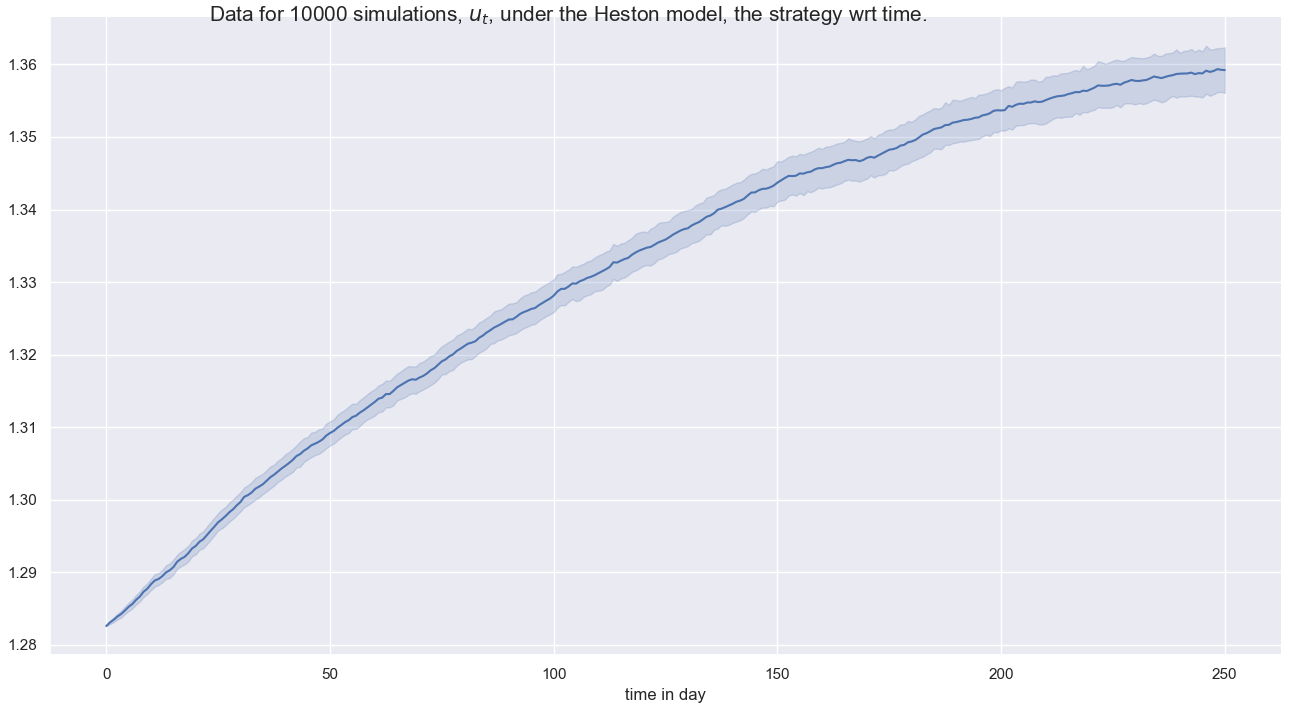
\includegraphics[width = 0.44 \textwidth]{../addition_part/images/numerical_studies/bootstrap_u_t.png}
}}
\subfloat{{
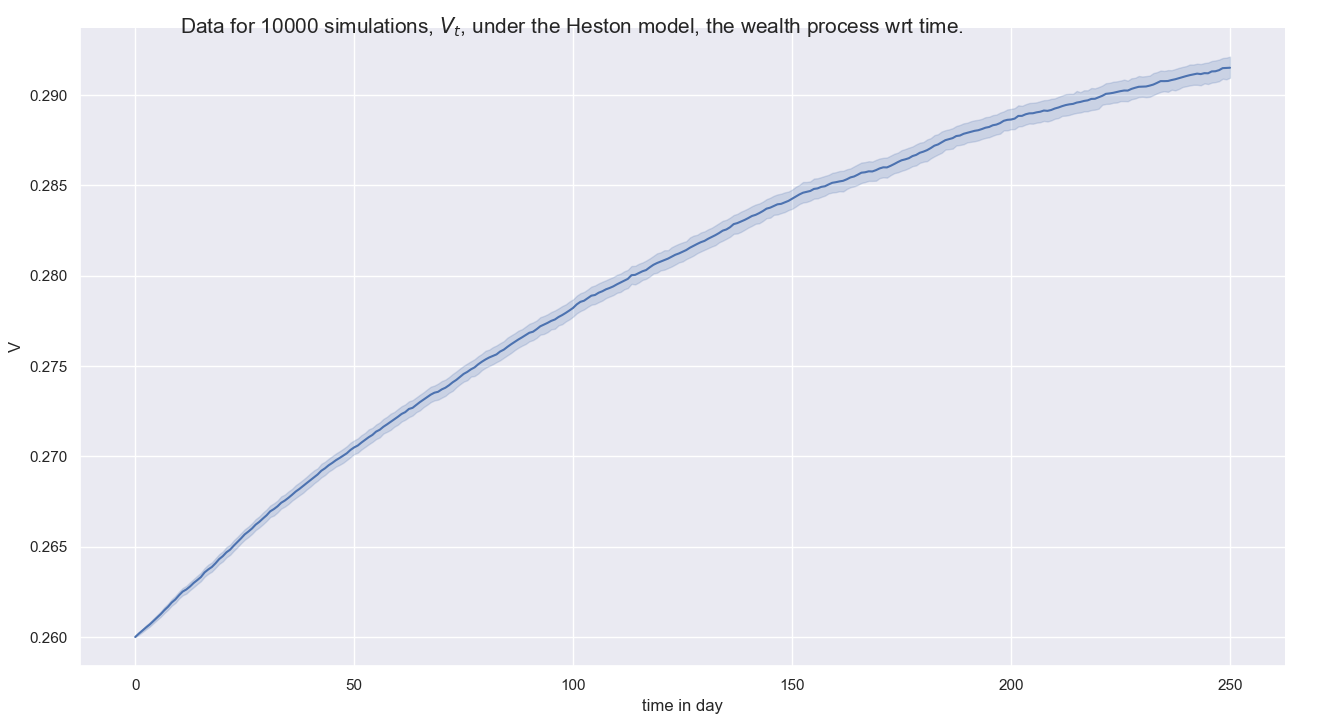
\includegraphics[width = 0.44 \textwidth]{../addition_part/images/numerical_studies/bootstrap_V_t.png}
}}\\
\subfloat{{
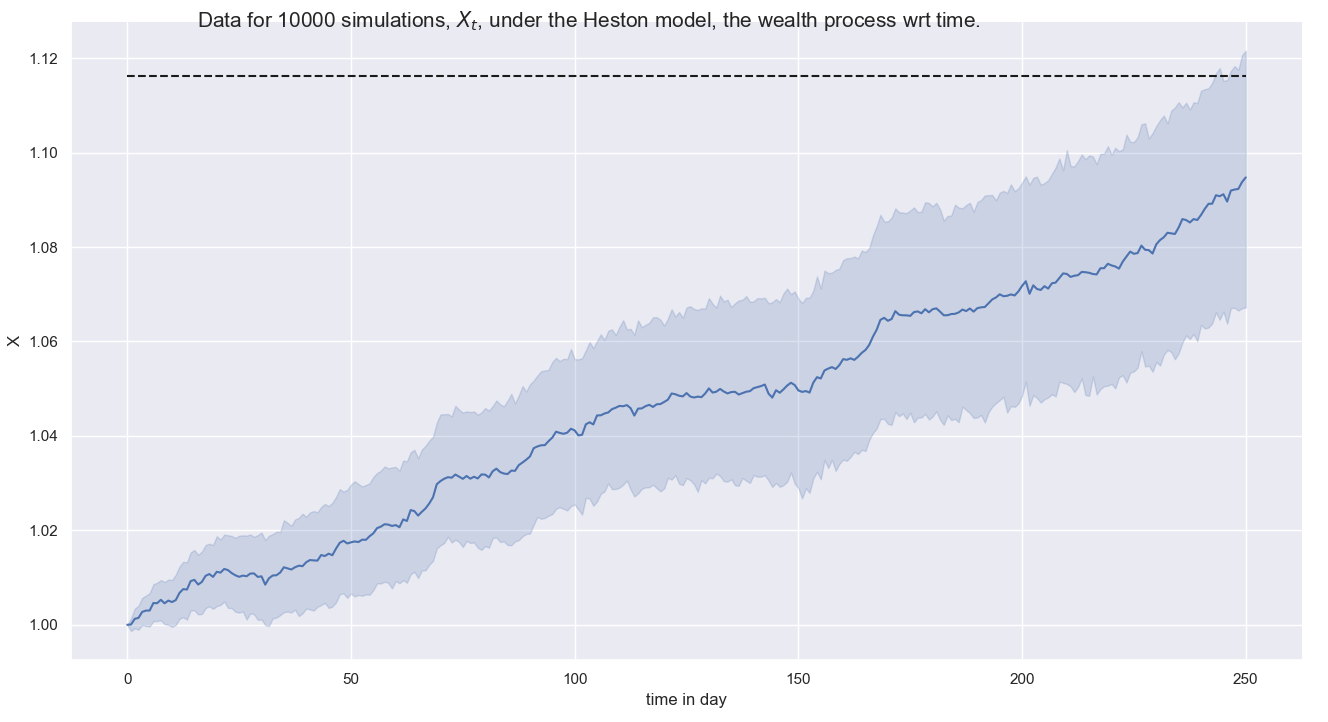
\includegraphics[width = 0.6 \textwidth]{../addition_part/images/numerical_studies/bootstrap_X_t.png}
}} 
\caption{Bootstrap of $10000$ simulations of the normal Heston, displaying the optimal strategy, the volatility, and the wealth.  Set of parameters nb. 1 in \ref{tab:bootstrap}.}
\label{fig:bootstrap}
\end{figure}





\begin{figure}[h]
\centering
\subfloat{{
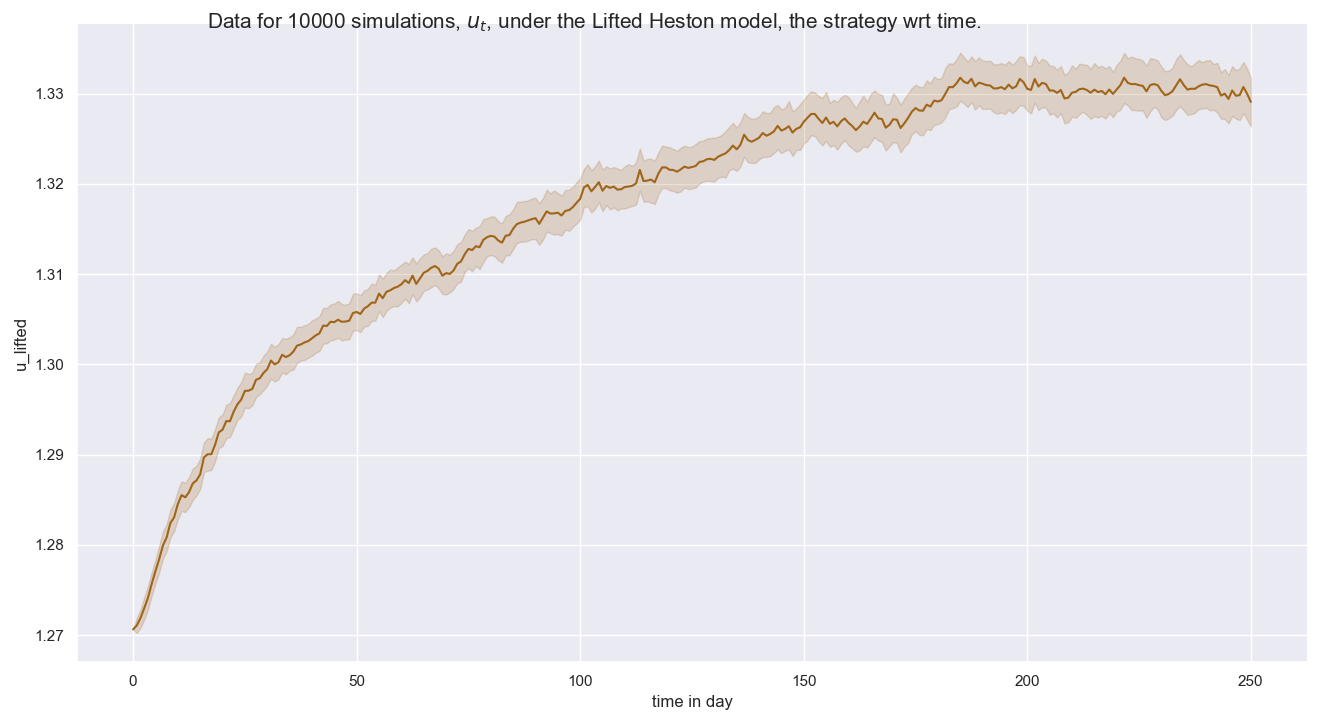
\includegraphics[width = 0.44 \textwidth]{../addition_part/images/numerical_studies/bootstrap_u_t_lifted.png}
}}
\subfloat{{
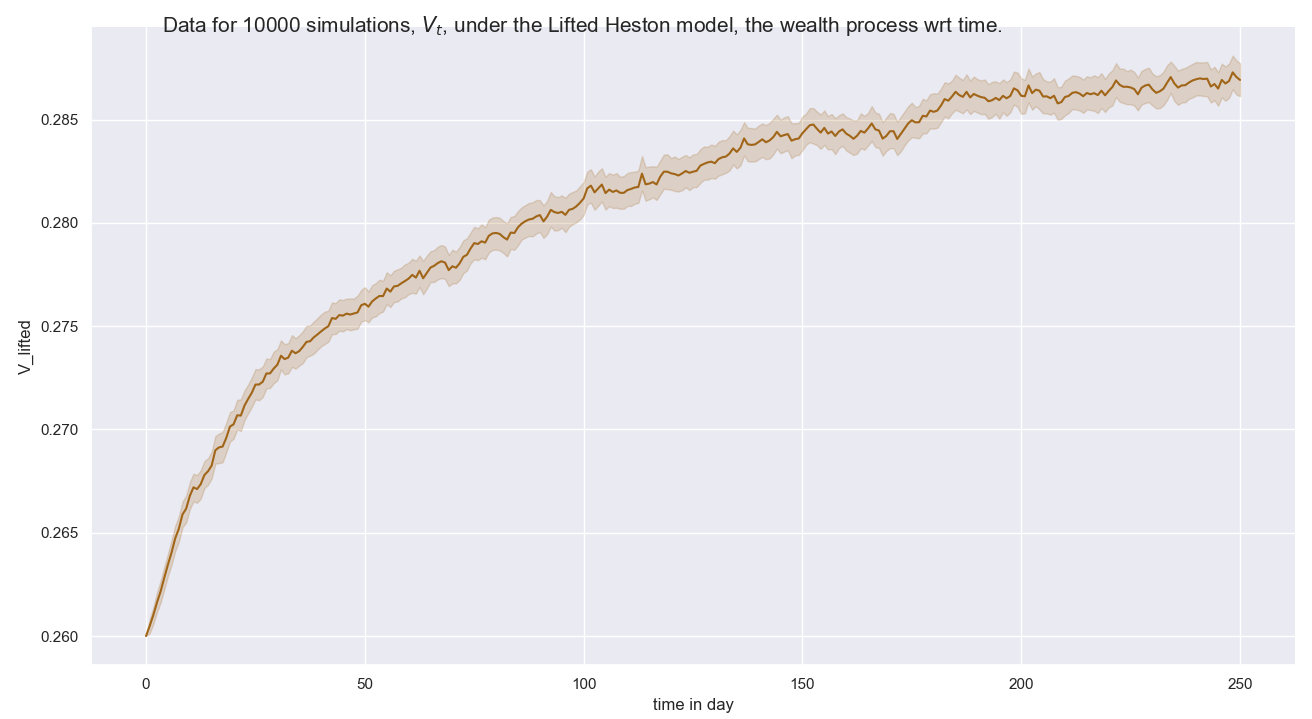
\includegraphics[width = 0.44 \textwidth]{../addition_part/images/numerical_studies/bootstrap_V_t_lifted.png}
}}\\
\subfloat{{
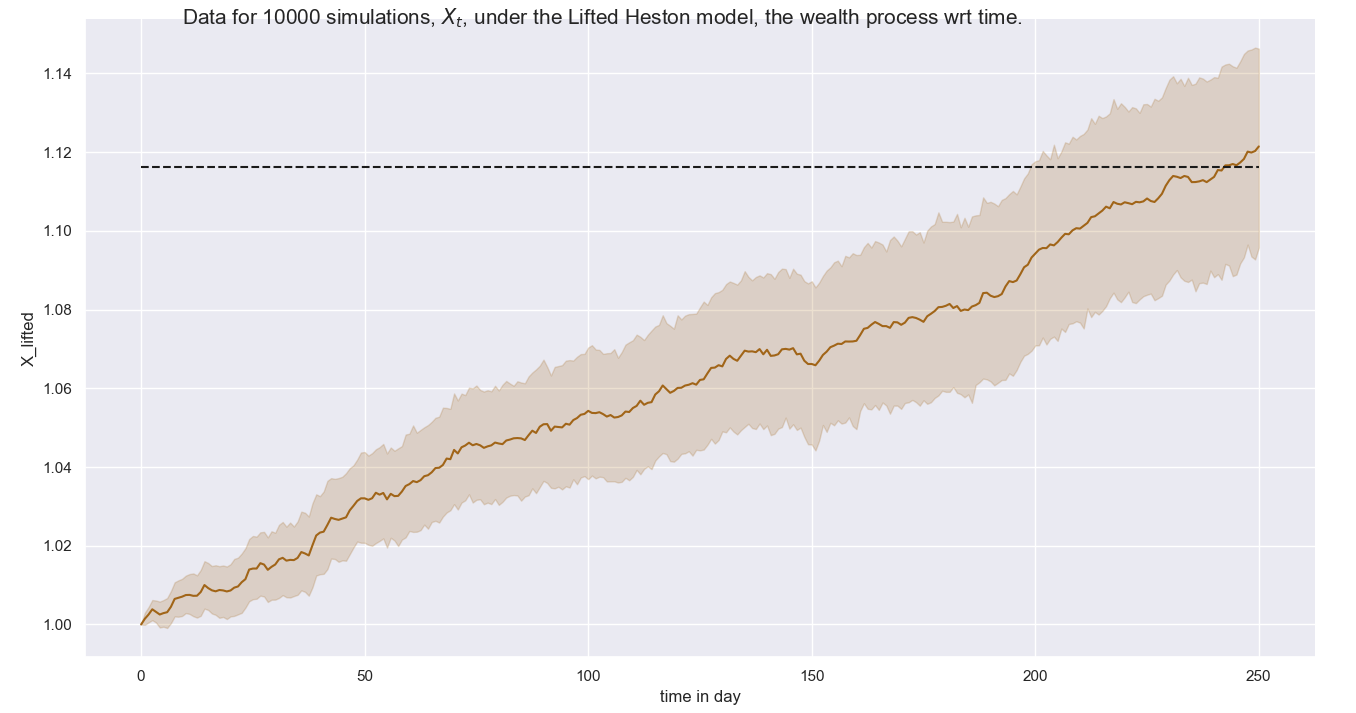
\includegraphics[width = 0.6 \textwidth]{../addition_part/images/numerical_studies/bootstrap_X_t_lifted.png}
}} 
\caption{Bootstrap of $10000$ simulations of the lifted Heston, $\alpha = 0.6 $, displaying the optimal strategy, the volatility, and the wealth. Set of parameters nb. 1 in \ref{tab:bootstrap}.}
\label{fig:bootstraplifted}
\end{figure}





\begin{figure}[h]
\centering
\subfloat{{
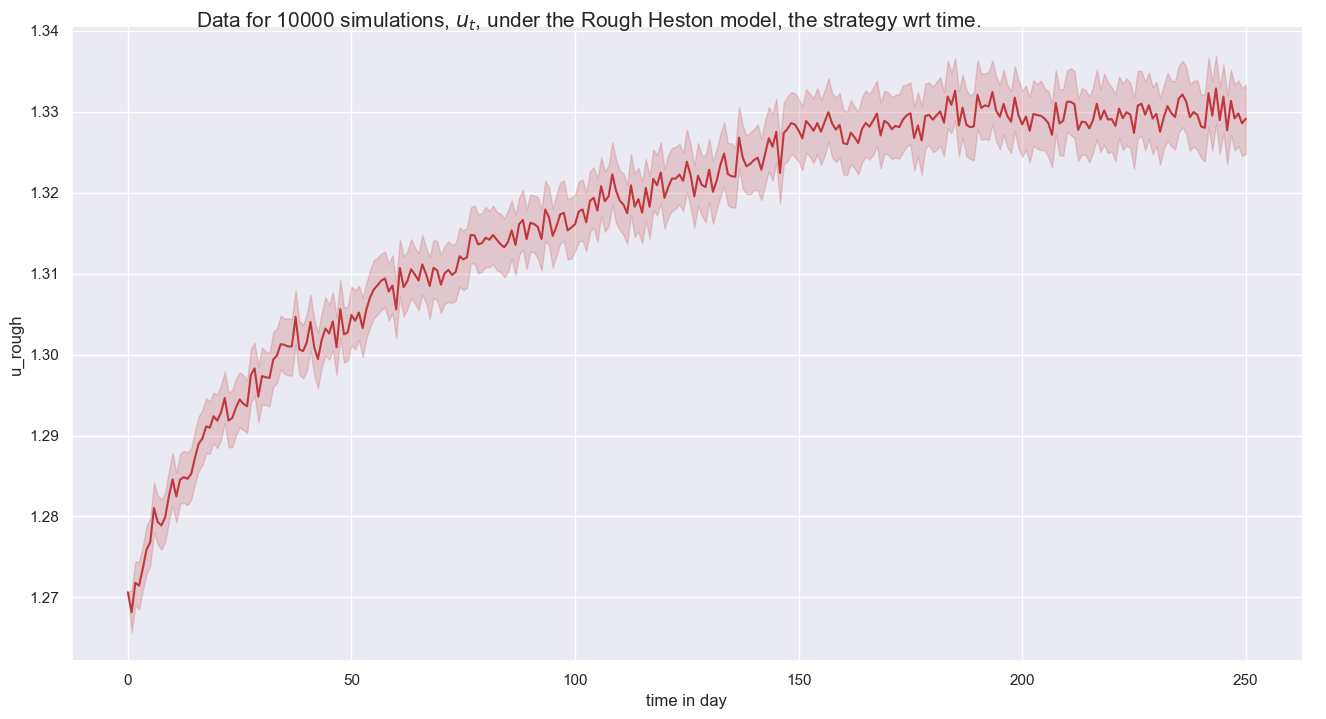
\includegraphics[width = 0.44 \textwidth]{../addition_part/images/numerical_studies/bootstrap_u_t_rough.png}
}}
\subfloat{{
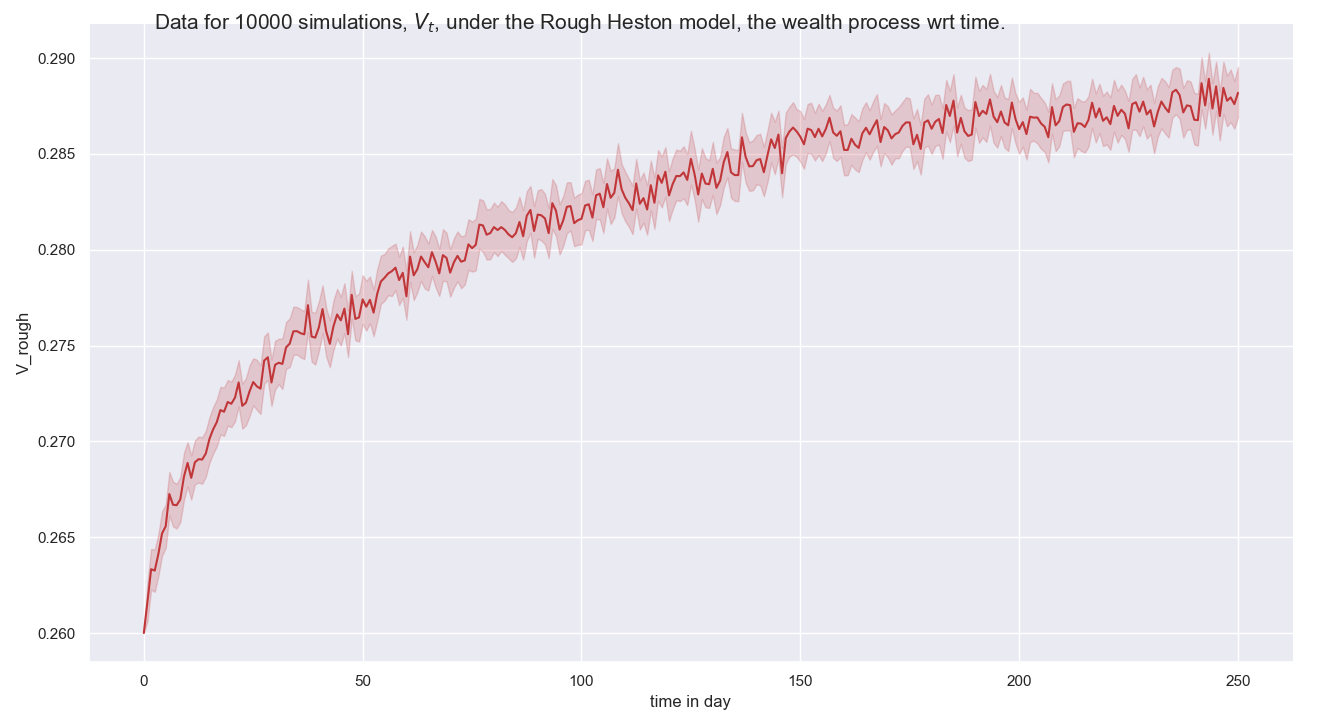
\includegraphics[width = 0.44 \textwidth]{../addition_part/images/numerical_studies/bootstrap_V_t_rough.png}
}}\\
\subfloat{{
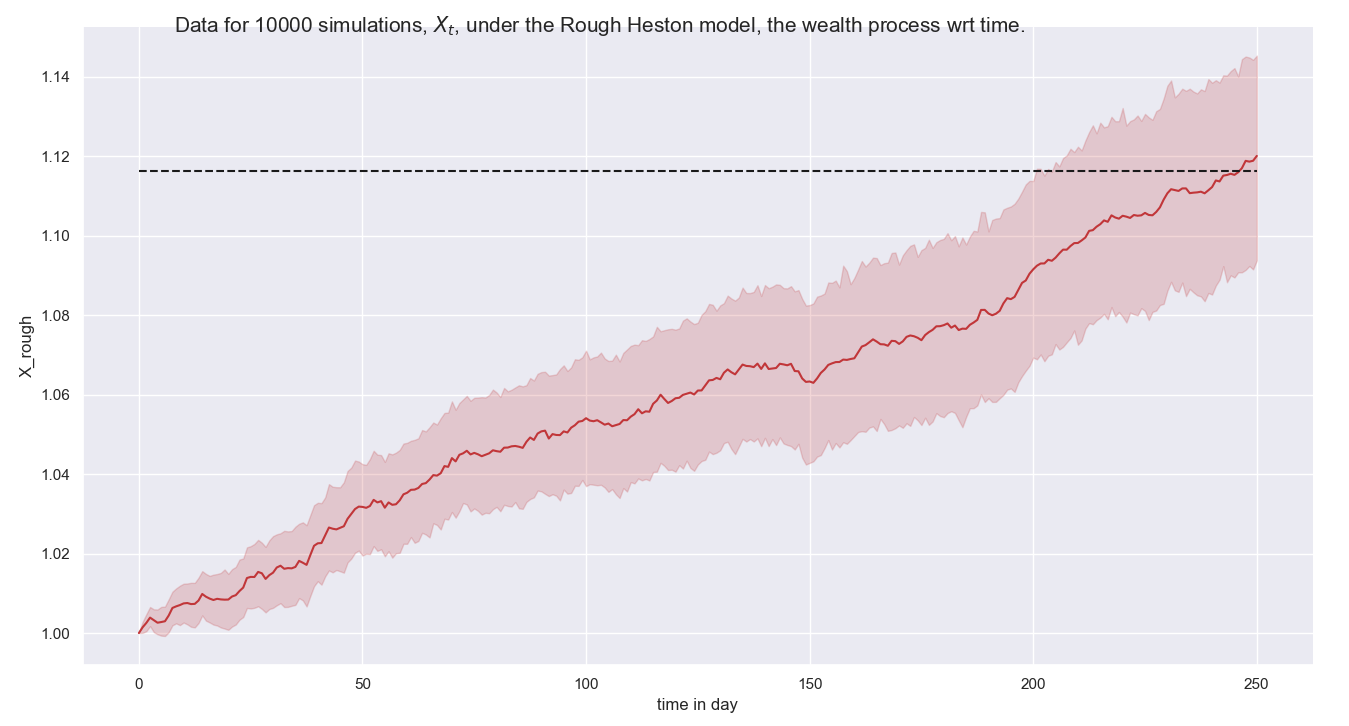
\includegraphics[width = 0.6 \textwidth]{../addition_part/images/numerical_studies/bootstrap_X_t_rough.png}
}} 
\caption{Bootstrap of $10000$ simulations of the rough Heston, $\alpha = 0.6 $, displaying the optimal strategy, the volatility, and the wealth. Set of parameters nb. 1 in \ref{tab:bootstrap}.}
\label{fig:bootstraprough}
\end{figure}




























\begin{figure}[h]
\centering
\subfloat{{
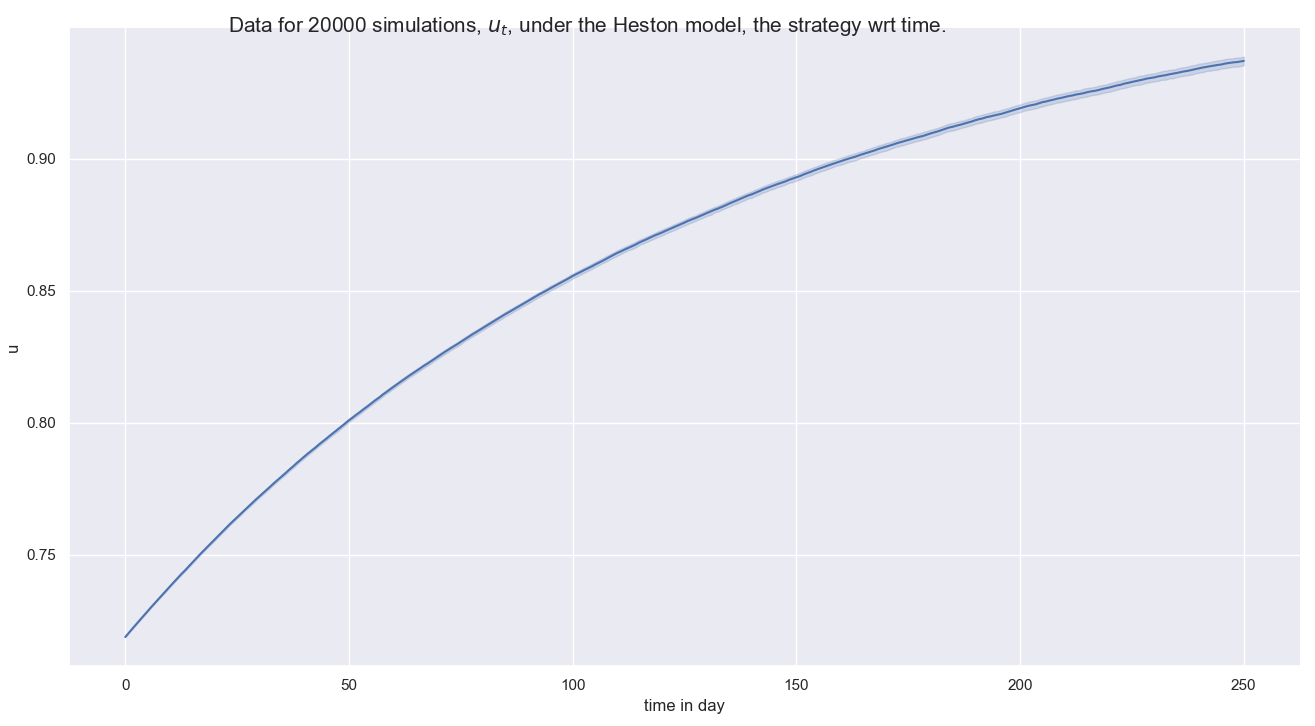
\includegraphics[width = 0.44 \textwidth]{../addition_part/images/numerical_studies/bootstrap_u_t2.png}
}}
\subfloat{{
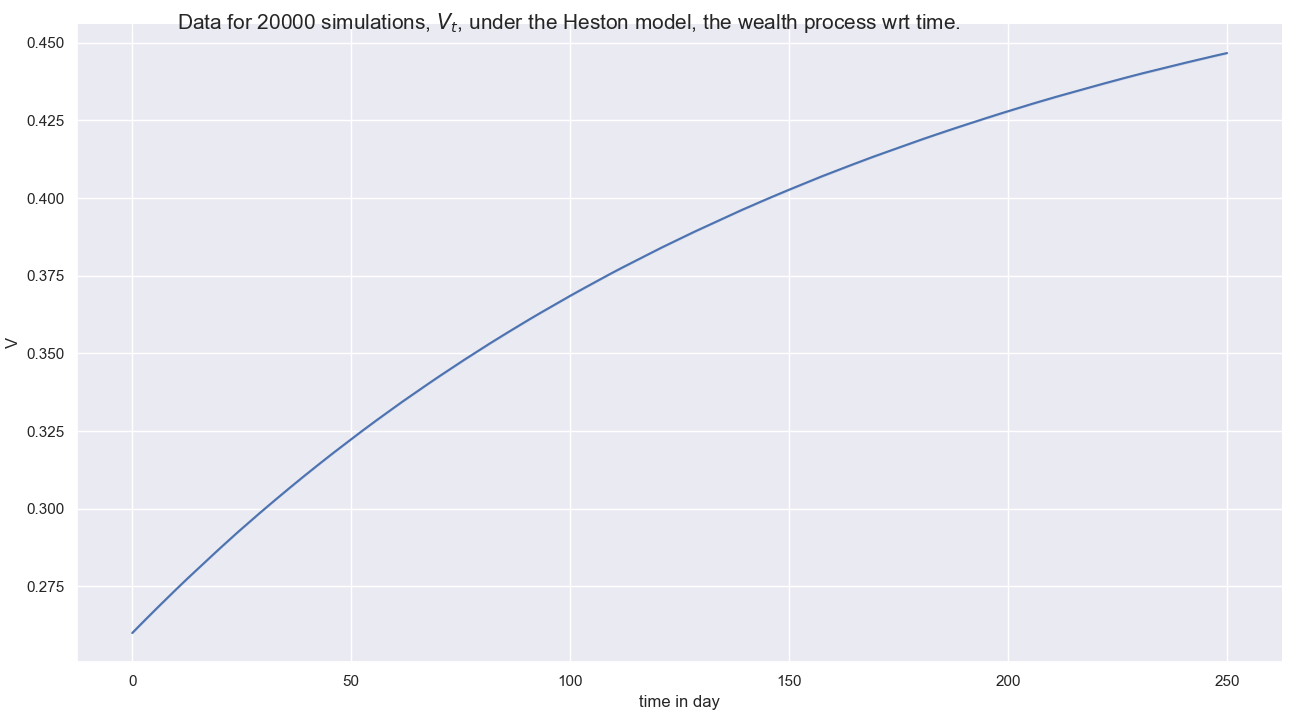
\includegraphics[width = 0.44 \textwidth]{../addition_part/images/numerical_studies/bootstrap_V_t2.png}
}}\\
\subfloat{{
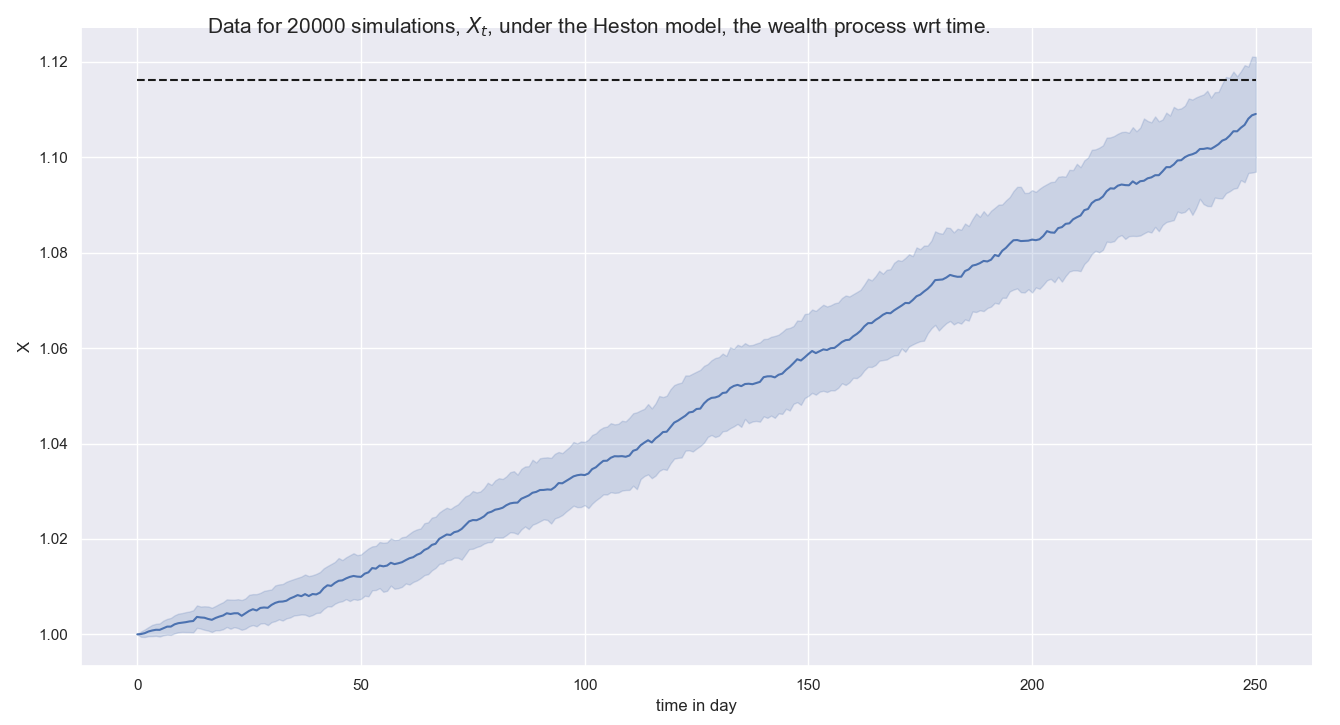
\includegraphics[width = 0.6 \textwidth]{../addition_part/images/numerical_studies/bootstrap_X_t2.png}
}} 
\caption{Bootstrap of $20000$ simulations of the normal Heston, displaying the optimal strategy, the volatility, and the wealth. Set of parameters nb. 2 in \ref{tab:bootstrap}.}
\label{fig:bootstrap2}
\end{figure}





\begin{figure}[h]
\centering
\subfloat{{
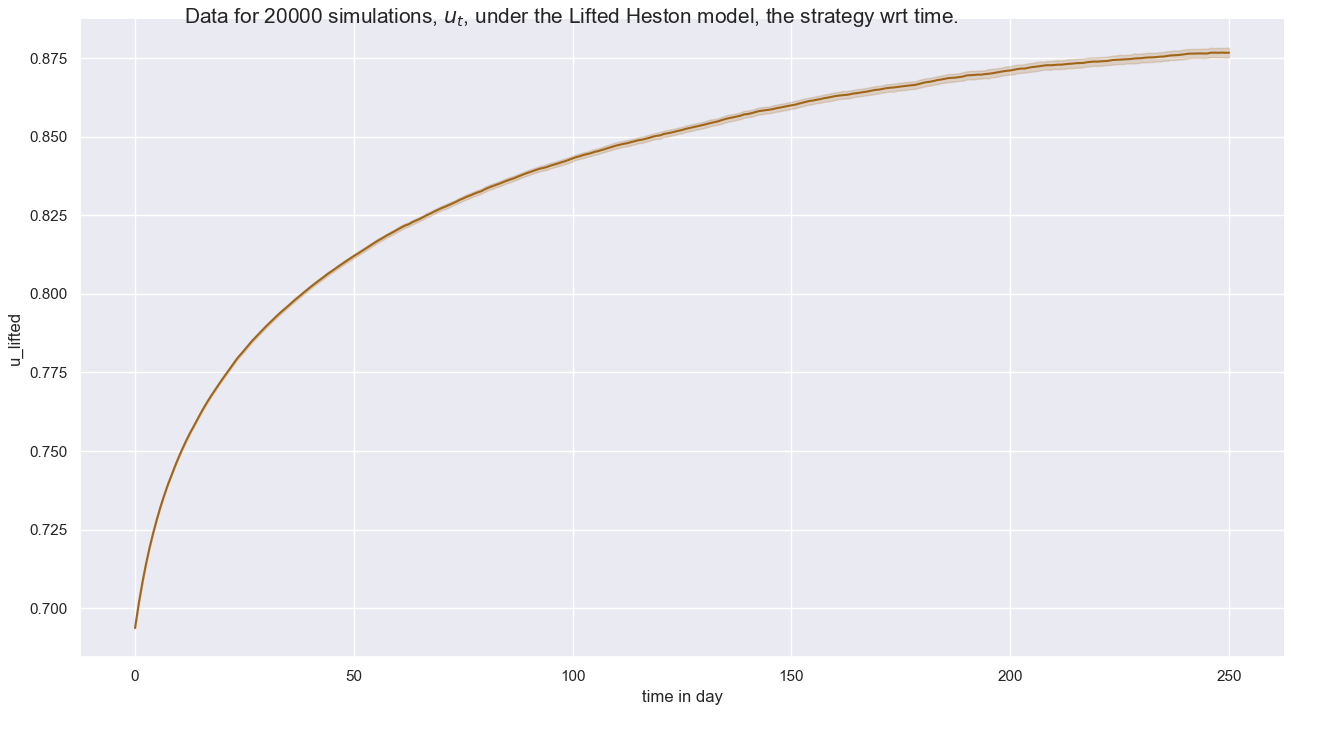
\includegraphics[width = 0.44 \textwidth]{../addition_part/images/numerical_studies/bootstrap_u_t_lifted2.png}
}}
\subfloat{{
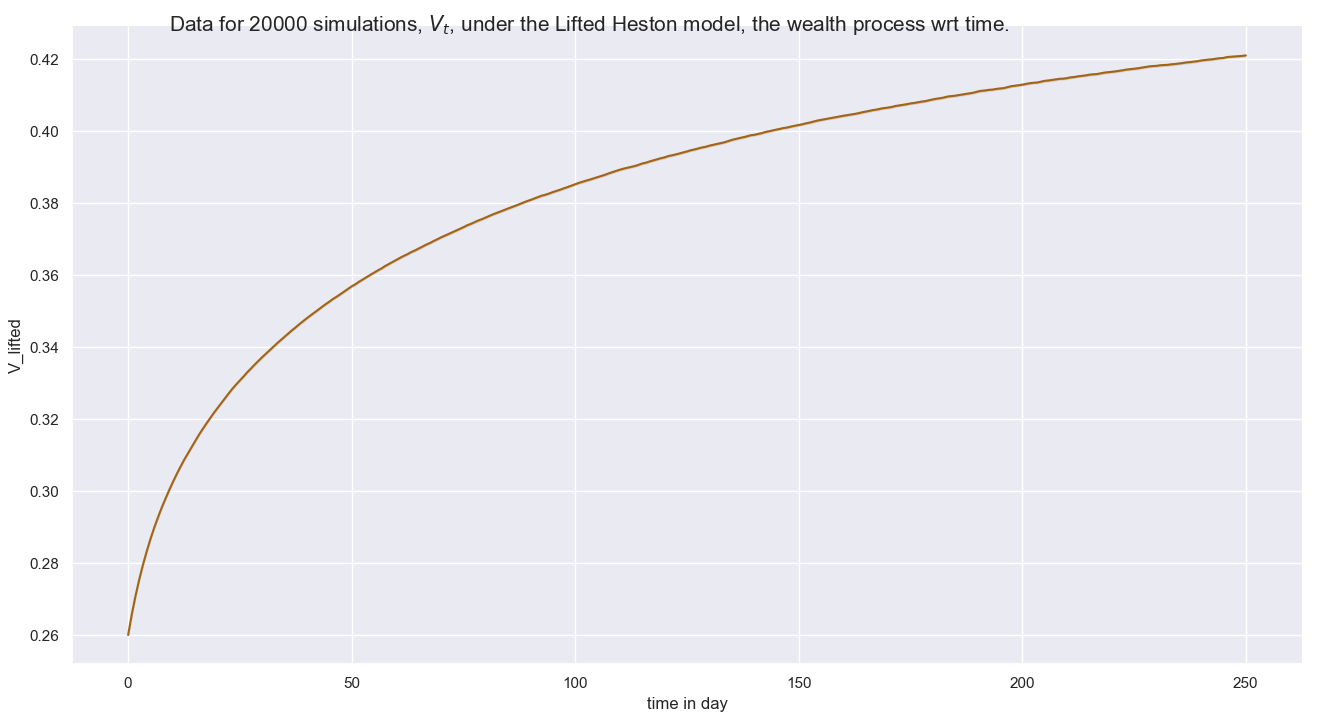
\includegraphics[width = 0.44 \textwidth]{../addition_part/images/numerical_studies/bootstrap_V_t_lifted2.png}
}}\\
\subfloat{{
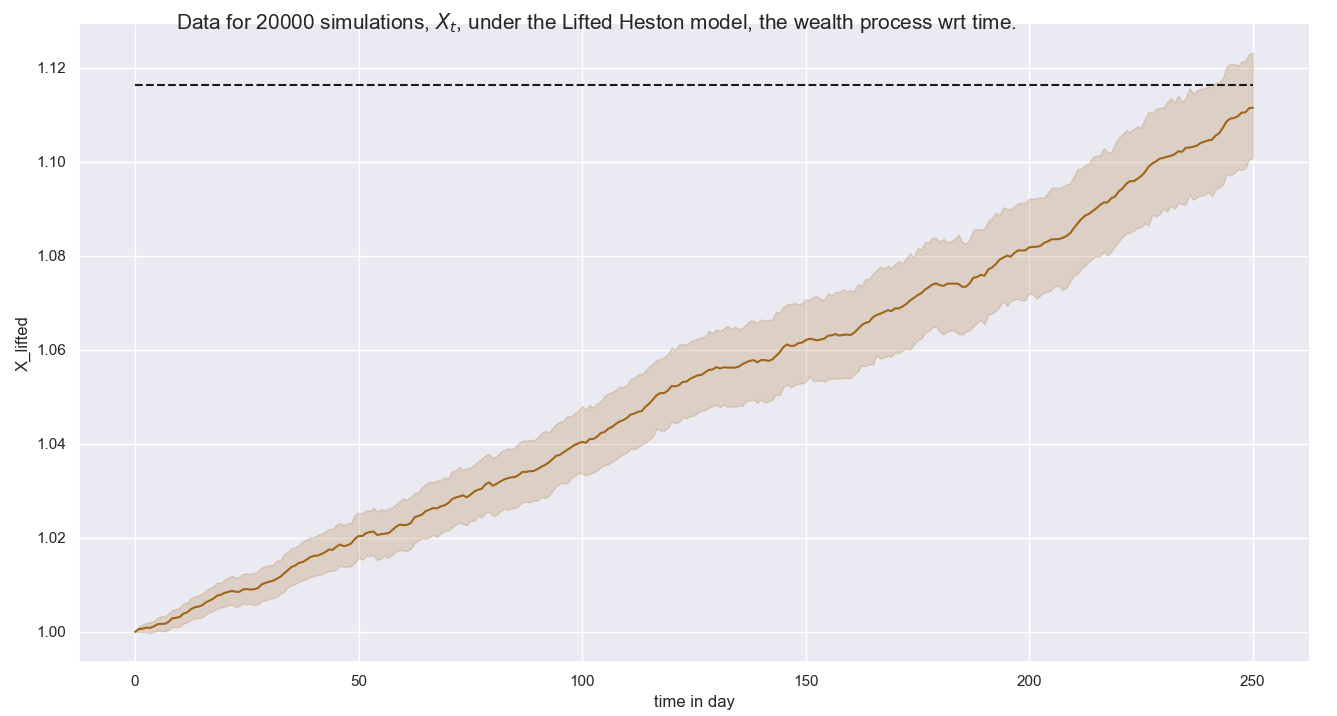
\includegraphics[width = 0.6 \textwidth]{../addition_part/images/numerical_studies/bootstrap_X_t_lifted2.png}
}} 
\caption{Bootstrap of $20000$ simulations of the lifted Heston, $\alpha = 0.6 $, displaying the optimal strategy, the volatility, and the wealth. Set of parameters nb. 2 in \ref{tab:bootstrap}.}
\label{fig:bootstraplifted2}
\end{figure}





\begin{figure}[h]
\centering
\subfloat{{
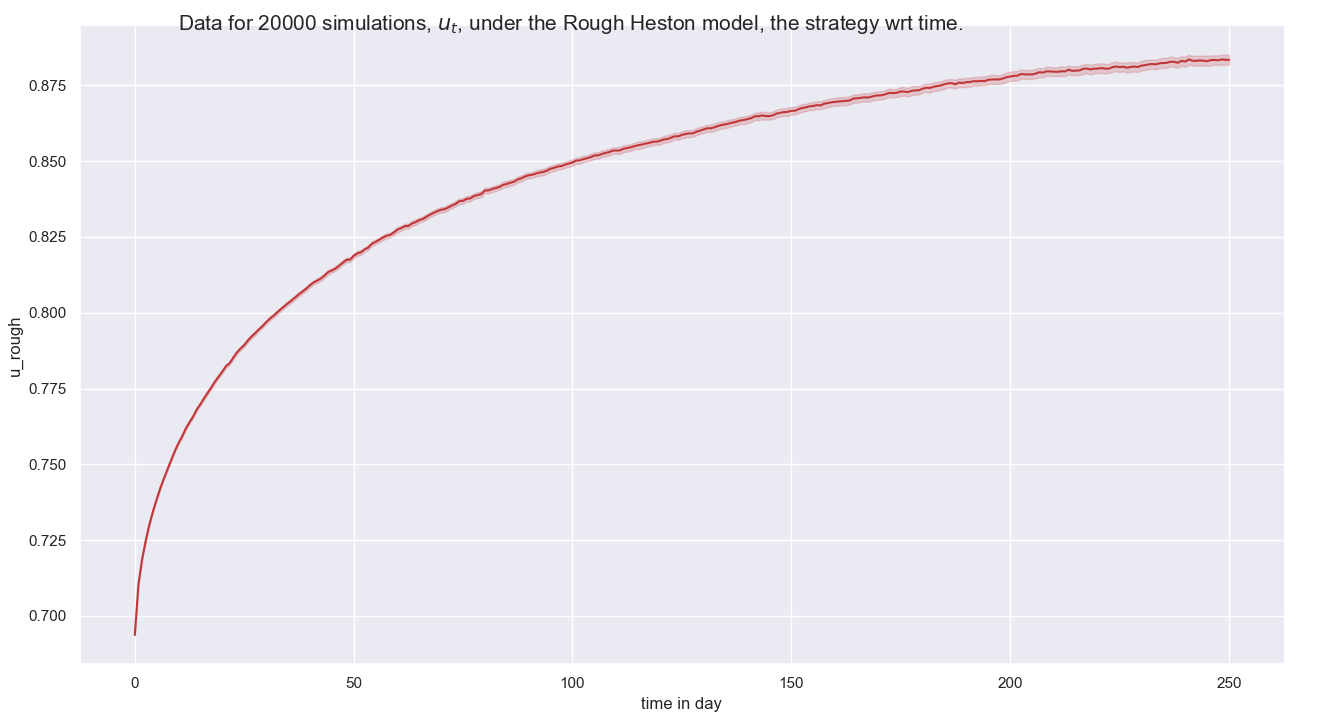
\includegraphics[width = 0.44 \textwidth]{../addition_part/images/numerical_studies/bootstrap_u_t_rough2.png}
}}
\subfloat{{
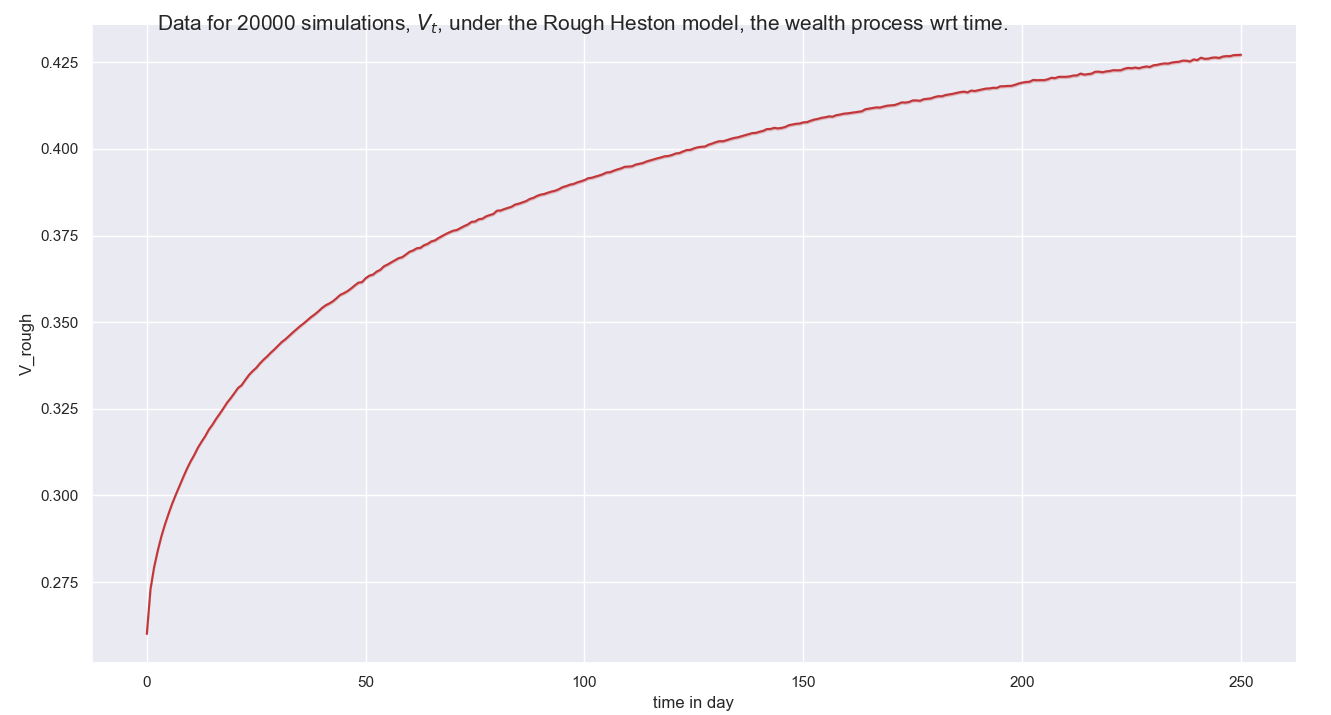
\includegraphics[width = 0.44 \textwidth]{../addition_part/images/numerical_studies/bootstrap_V_t_rough2.png}
}}\\
\subfloat{{
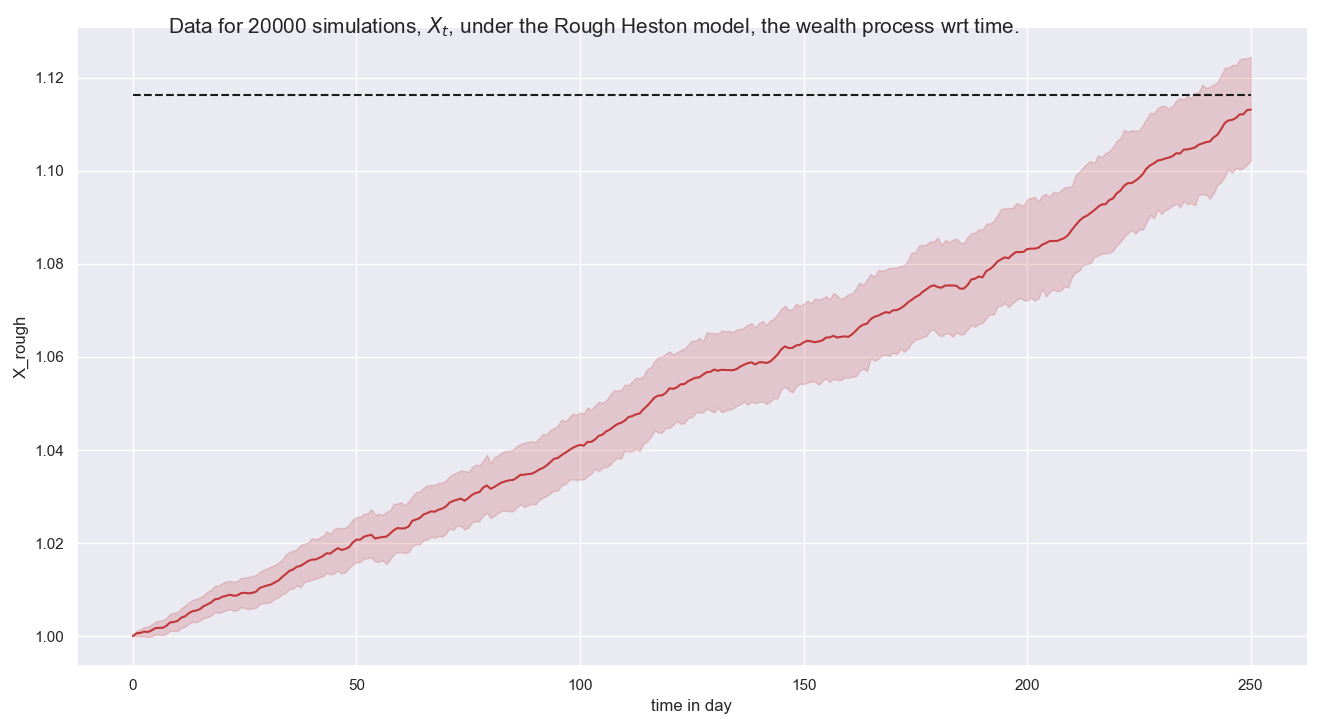
\includegraphics[width = 0.6 \textwidth]{../addition_part/images/numerical_studies/bootstrap_X_t_rough2.png}
}} 
\caption{Bootstrap of $20000$ simulations of the rough Heston, $\alpha = 0.6 $, displaying the optimal strategy, the volatility, and the wealth. Set of parameters nb. 2 in \ref{tab:bootstrap}.}
\label{fig:bootstraprough2}
\end{figure}


\begin{remarque}
In addition to the previous optimistic results, I have also observed that they are heavily dependent on the parameters, and sometimes luck. When $\theta$ is too small, the optimal investment becomes quite instable (due to the fact that the solution to $\psi$ is not that precise anymore) and so the wealth under the classical Heston model fluctuates a lot and does not grow. Also, even though I simulated a big number of paths (20 000), sometimes the results can change from a seed to another, and one gets more payoff from the normal model than from the rough models. 
\end{remarque}

\begin{remarque}
Also, we see on fig. \ref{fig:bootstraplifted} and fig. \ref{fig:bootstraprough} that the expected wealth is higher than the target. It is  for the simple reason that we are simulating the wealth and there is some variance associated to it.
\end{remarque}

\begin{remarque}
Finally, we observe more payoff from Mr. Jacquier's rough model, than from the lifted version, certainly because the former is rougher than the latter.
\end{remarque}


\subsection{Forward Variance }

Forward Variance is a topic I barely scratched. A scheme for simulating it under rough Heston is proposed in \cite{ROUGH_HESTON}.

Here, I will simply recall the definition of it, and give its expression under the Heston model.

\begin{definition}[Forward Variance]
For a process which dynamics is given by the Volterra-Heston equation, with $b_s$ as drift and $\sigma_s$ the volatility, then:
$$ \Theta_u^t := \E \left [ V_u  - 1_{ t \leq u } \cdot  \int_t^u b_s ds  | \mathcal F_t  \right ] $$
\end{definition}

In other words, it is the mean of the expected variance knowing a future state of the world. If one fixes $u < t$, then the forward variance $\Theta_u^t$ reduces to $V_u$.











